% =====================================================================
% Mirante dos Dados — Working Paper #7
% 5.570 Pontos de Decisão: Microdados Municipais do Bolsa Família,
% Identificação Causal por Variação Cross-Municipal e Heterogeneidade
% Intra-UF (2013–2025)
%
% Autor: Leonardo Chalhoub
% Versão: 1.0 — Abril de 2026 (resposta direta ao gargalo de N=27 clusters
%        identificado na peer review do WP#2 em 2026-04-27).
%        Conley HAC sobre lat/lon real (IBGE Localidades + kelvins/MB);
%        TWFE com k≈5.570 clusters; DiD em duas rupturas; decomposição
%        Theil within/between-UF; sub-atendimento intra-UF.
% Compilação: pdflatex articles/bolsa-familia-municipios.tex (2x)
% =====================================================================

\documentclass[12pt,a4paper,oneside]{article}

\usepackage[T1]{fontenc}
\usepackage[utf8]{inputenc}
\usepackage[brazilian]{babel}
\usepackage{newtxtext}
\usepackage{newtxmath}
\usepackage[section]{placeins}
\usepackage[a4paper,top=3cm,bottom=2cm,left=3cm,right=2cm]{geometry}
\usepackage{setspace}
\usepackage{indentfirst}
\usepackage{titlesec}
\usepackage{caption}
\usepackage{booktabs}
\usepackage{array}
\usepackage{multirow}
\usepackage{graphicx}
\usepackage[colorlinks=true,
            urlcolor=blue!60!black,
            linkcolor=black,
            citecolor=black,
            breaklinks=true]{hyperref}
\usepackage{url}
\usepackage{xurl}
\Urlmuskip=0mu plus 1mu\relax
\usepackage{float}
\usepackage{tcolorbox}

\graphicspath{{figures-pbf-municipios/}}

\onehalfspacing
\setlength{\parindent}{1.25cm}
\setlength{\parskip}{0pt}

\titleformat{\section}{\normalfont\bfseries\large\uppercase}{\thesection}{0.6em}{}
\titleformat{\subsection}{\normalfont\bfseries\normalsize}{\thesubsection}{0.6em}{}
\titlespacing*{\section}{0pt}{18pt}{8pt}
\titlespacing*{\subsection}{0pt}{12pt}{6pt}

\captionsetup[table]{labelfont=bf,name=Tabela,labelsep=endash,
                     position=above,justification=centering,font=small}
\captionsetup[figure]{labelfont=bf,name=Figura,labelsep=endash,
                      position=below,justification=centering,font=small}
\captionsetup{skip=6pt}

\newcommand{\rs}{R\$\,}

% Stamp de compilação injetado pelo CI (deploy-pages.yml).
% Para builds locais, este arquivo default é usado — basta um pdflatex direto
% e a capa exibe "(dev local)". Em CI, este arquivo é sobrescrito antes da
% compilação com timestamp BRT + SHA do commit que disparou o deploy.
\newcommand{\COMPILESTAMP}{compila\c{c}\~ao local}
\newcommand{\COMPILESHA}{dev}


\begin{document}

% ---------- CAPA ---------------------------------------------------------
\begin{titlepage}
  \begin{center}
    \vspace*{1.5cm}
    {\small\textsc{Mirante dos Dados \quad\textbar\quad Working Paper n. 7}}\\
    {\small Versão 1.0 \textemdash{} Abril de 2026}\\[2pt]
    {\footnotesize Compilada em \COMPILESTAMP\ \textbullet\ \texttt{\COMPILESHA}}

    \vfill

    {\LARGE\bfseries
     5.570 PONTOS DE DECISÃO:

     MICRODADOS MUNICIPAIS DO
     BOLSA FAMÍLIA,

     IDENTIFICAÇÃO CAUSAL POR
     VARIAÇÃO CROSS-MUNICIPAL E

     HETEROGENEIDADE INTRA-UF
     (2013\textendash 2025)}

    \vspace{1cm}
    {\large\itshape
     5{,}570 decision points: municipal microdata of Brazil's Bolsa
     Família, causal identification via cross-municipal variation and
     within-state heterogeneity (2013\textendash 2025)}

    \vfill

    {\large\textbf{Leonardo Chalhoub}}\\[4pt]
    {\small Pesquisador independente \textemdash{} engenharia de dados,
     análise quasi-experimental espacialmente robusta,
     decomposição de desigualdade.}\\[2pt]
    {\small\href{mailto:leonardochalhoub@gmail.com}{leonardochalhoub@gmail.com}}\\
    {\small\href{https://github.com/leonardochalhoub/mirante-dos-dados-br}{github.com/leonardochalhoub/mirante-dos-dados-br}}

    \vfill

    {\small Brasil \\ Abril de 2026}
  \end{center}
\end{titlepage}

% ---------- RESUMO -------------------------------------------------------
\section*{Resumo}
\addcontentsline{toc}{section}{Resumo}
\begin{singlespace}\small\noindent
Sobre o Bolsa Família no período 2013\textendash 2025 com granularidade
\textbf{municipal} (5{,}570 unidades), este trabalho responde diretamente
ao gargalo identificacional identificado pela revisão de pares interna
do trabalho companheiro sobre o programa em painel UF\,$\times$\,Ano:
\textbf{N\,=\,27 clusters de UF é insuficiente para que estimadores
cluster-robustos como o \textit{wild-cluster bootstrap} de Cameron,
Gelbach e Miller (2008) convirjam}. \textbf{Materiais e métodos.} A
análise integra (i) o painel CGU/Portal da Transparência consolidado em
arquitetura medallion (bronze \textrightarrow{} silver \textrightarrow{}
gold) com agregação Município\,$\times$\,Ano (\,2{,}5\,bilhões de linhas
de microdados PBF\,/\,Auxílio Brasil\,/\,Novo Bolsa Família reduzidos a
um painel de \,$\sim$\,72{,}000 linhas\,); (ii) coordenadas geodésicas
oficiais do IBGE\,/\,Localidades + kelvins\,/\,Municipios-Brasileiros
para 5{,}570 centroides; (iii) população residente estimada
IBGE\,/\,SIDRA Tabela 6579 (variável 9324) por município\,$\times$\,ano,
com extrapolação linear para 2022\,/\,2023 (anos do Censo sem
publicação); (iv) deflação IPCA-BCB base dezembro\,/\,2021. A
identificação causal articula \textbf{quatro estratégias
complementares}: (i) \textit{difference-in-differences} 2\,$\times$\,2
sobre a Medida Provisória n.\,1.061\,/\,2021 (Auxílio Brasil) e a Lei
n.\,14.601\,/\,2023 (Novo Bolsa Família), com tratamento na intensidade
municipal do \textit{déficit de cobertura} pré-choque
(pobreza\,$-$\,penetração); (ii) modelo \textit{two-way fixed effects}
(TWFE) com efeitos fixos de município e ano e erros clusterizados por
município ($k = 5{,}570$, vinte vezes acima do mínimo recomendado por
Cameron-Gelbach-Miller); (iii) \textit{Conley HAC} (Conley, 1999) com
distâncias geodésicas haversine reais entre centroides e bandwidth
sensitivity analysis em $\{50, 100, 200, 400, 800, 1600\}$\,km, que
captura correlação espacial residual sem depender de partição
arbitrária em \textit{clusters}; (iv) \textit{event study} com
\textit{leads} e \textit{lags} para diagnóstico visual de
\textit{parallel trends} no painel municipal. A decomposição da
desigualdade do PBF per capita em \textit{within-UF} e
\textit{between-UF} via índice de Theil L (\textit{mean log
deviation}) quantifica quanto da variação ocorre dentro de UFs
\textemdash{} e portanto é invisível em análises agregadas em UF. A
distribuição cumulativa dos 5{,}570 munis (\textit{curva de Lorenz}
municipal) caracteriza a focalização espacial efetiva do programa.
\textbf{Achados.} A migração para granularidade municipal reduz o erro
padrão \textit{cluster}-robusto em ordem de magnitude
($\hat{\beta}_{\text{TWFE}} = +297$\,\rs/hab; $SE_{\text{cluster}} =
2{,}56$; $t = 115{,}7$; $n = 44{,}568$; $k = 5{,}571$\,municípios). A
sensibilidade Conley-HAC ao \textit{bandwidth} é, contudo, expressiva:
$SE$ infla de 10{,}9 (50\,km) a 149{,}2 (1\,600\,km), evidenciando
correlação espacial positiva substancial nos resíduos. Sob
\textit{bandwidth} de 1\,600\,km \textemdash{} suficiente para conter a
maior parte das interações vizinho-vizinho \textemdash{} o efeito
permanece estatisticamente diferente de zero ($t \approx 2{,}0$). O
\textit{difference-in-differences} 2\,$\times$\,2 sobre a MP
1.061\,/\,2021 produz $\hat{\beta} = +205{,}3$\,\rs/hab
(IC\,95\,\%~$[+201{,}2;\,+209{,}3]$, $p < 0{,}001$ no \textit{cluster
bootstrap} por município, $k = 5{,}571$); a replicação cross-shock
sobre a Lei 14.601\,/\,2023 produz $\hat{\beta} = +349{,}5$\,\rs/hab
(IC\,95\,\%~$[+343{,}9;\,+355{,}2]$, $p < 0{,}001$). A magnitude maior
do segundo coeficiente é consistente com o redesenho do NBF (piso
\rs\,600 + adicionais por composição) ter um componente vertical
adicional ao da MP 1.061. A decomposição Theil mostra que a parcela
\textit{within-UF} da desigualdade municipal do PBF per capita é
substancial \textemdash{} médias estaduais escondem variação interna
não-trivial. \textbf{Discussão e contribuição.} O trabalho publica
abertamente: (i) os \textit{notebooks} Databricks da arquitetura
\textit{lakehouse} para agregação Município\,$\times$\,Ano dos 2{,}5\,bi
de linhas do bronze CGU; (ii) o \textit{fallback gold} local com
extrapolação linear documentada para anos sem publicação IBGE; (iii) o
\textit{script} de análise causal com TWFE clusterizado, Conley HAC
simulado e \textit{event study}. A contribuição metodológica central é
demonstrar a \textbf{viabilidade prática} de identificação causal
espacialmente robusta sobre programas sociais brasileiros usando os
microdados municipais já abertos pela CGU \textemdash{} reduzindo o
custo marginal de pesquisa quasi-experimental sobre o programa de
meses-de-engenharia para minutos-de-leitura.

\vspace{0.4cm}\noindent\textbf{Palavras-chave:}
Programa Bolsa Família; Auxílio Brasil; Novo Bolsa Família;
microdados municipais; identificação causal espacialmente robusta;
\textit{Conley HAC}; \textit{two-way fixed effects}; \textit{cluster
bootstrap}; decomposição Theil within\,/\,between; heterogeneidade
intra-UF; arquitetura medallion; \textit{lakehouse}.
\end{singlespace}

% ---------- ABSTRACT -----------------------------------------------------
\section*{Abstract}
\addcontentsline{toc}{section}{Abstract}
\begin{singlespace}\small\noindent
This paper provides a direct response to the small-cluster bottleneck
flagged in the internal peer review of the companion working paper on
Brazil's Bolsa Família at the state\,$\times$\,year level: with
$N = 27$ states, the cluster-robust \textit{wild-cluster bootstrap}
(Cameron, Gelbach \& Miller, 2008) does not converge reliably.
\textbf{Methods.} We migrate the panel to municipal granularity
(5{,}570 units), consolidating CGU's microdata via a medallion
architecture (bronze\,$\rightarrow$\,silver\,$\rightarrow$\,gold), with
geodesic centroids from IBGE/Localidades + kelvins/Municipios-Brasileiros,
population from IBGE/SIDRA Table~6579 (with linear extrapolation for the
2022/2023 census years where IBGE did not publish estimates), and IPCA
deflation (December~2021). Causal identification combines (i) DiD
2\,$\times$\,2 on Provisional Measure 1.061/2021 (Auxílio Brasil) and
Law 14.601/2023 (Novo Bolsa Família) with treatment intensity defined by
the pre-shock municipal coverage \textit{deficit} (poverty $-$
penetration); (ii) two-way fixed effects with municipality and year
fixed effects and standard errors clustered by municipality
($k = 5{,}571$, twenty-fold above the recommended minimum); (iii)
\textit{Conley HAC} (Conley, 1999) with haversine distances and
bandwidth sensitivity in $\{50, 100, 200, 400, 800, 1600\}$\,km;
(iv)~event study with leads and lags. \textbf{Findings.} The
TWFE coefficient is $\hat{\beta} = +297$\,R\$ per capita
($SE_{\text{cluster}} = 2.56$; $t = 115.7$; $n = 44{,}568$). Conley HAC
sensitivity is substantial: $SE$ inflates from $10.9$ (50\,km) to
$149.2$ (1{,}600\,km). DiD 2\,$\times$\,2 on MP~1.061: $+205.3$\,R\$
per capita (95\,\%~CI~$[201.2;\,209.3]$, $p < 0.001$); on
Law~14.601/2023: $+349.5$\,R\$ per capita (95\,\%~CI~$[343.9;\,355.2]$,
$p < 0.001$). Theil decomposition shows substantial within-state
inequality, invisible at the UF level. \textbf{Discussion.} The paper
publishes the lakehouse pipelines, the local fallback gold, and the
causal analysis scripts \textemdash{} reducing the marginal cost of
quasi-experimental research on the program from months of engineering
to minutes of reading.

\vspace{0.4cm}\noindent\textbf{Keywords:}
Bolsa Família; Auxílio Brasil; Novo Bolsa Família; municipal microdata;
spatially-robust causal identification; Conley HAC; two-way fixed
effects; cluster bootstrap; Theil decomposition; within/between-state
heterogeneity; medallion architecture; lakehouse.
\end{singlespace}

\newpage

% ---------- SUMÁRIO + LISTAS --------------------------------------------
\renewcommand{\contentsname}{Sumário}
\tableofcontents

\newpage
\renewcommand{\listfigurename}{Lista de Figuras}
\listoffigures

\vspace{1cm}
\renewcommand{\listtablename}{Lista de Tabelas}
\listoftables

\newpage

% =====================================================================
\section{Introdução e motivação}\label{sec:intro}
% =====================================================================

A revisão de pares interna sobre o painel UF\,$\times$\,Ano do Bolsa
Família realizada em abril de 2026 explicitou um problema
metodológico central: \textbf{o número de \textit{clusters}
(N\,=\,27 UFs) é insuficiente para que o \textit{wild-cluster bootstrap}
de Cameron, Gelbach e Miller (2008) convirja de modo confiável}. Os
autores citados recomendam $k \geq 30$ \textit{clusters}, e o
desempenho do estimador degrada-se rapidamente abaixo desse limiar.
A consequência prática observada no painel UF\,$\times$\,Ano foi que o
$p$-valor robusto para o efeito da MP n.\,1.061\,/\,2021 sobre o PBF
per capita estadual divergiu drasticamente do $p$-valor naive HC3
($p_{\text{HC3}} < 0{,}001$ versus $p_{\text{WCB}} = 0{,}49$),
inviabilizando inferência confiável.

Este trabalho propõe uma solução metodológica direta: \textbf{migrar a
unidade de análise para o município}. O Brasil tem 5{,}570 municípios
com governos próprios, identificadores IBGE estáveis e cobertura
universal pelo CadÚnico/MDS, o que cria 5{,}570 \textit{clusters}
naturalmente disponíveis para inferência cluster-robusta. Com
$k \approx 5{,}570$, o problema dos poucos \textit{clusters}
desaparece. Adicionalmente, a granularidade municipal habilita técnicas
de identificação espacialmente robustas \textemdash{} notavelmente o
estimador \textit{Conley HAC} (Conley, 1999) com distâncias geodésicas
reais entre centroides \textemdash{} que são impossíveis com 27
\textit{clusters} de UF.

A migração não é trivial. O \textit{bronze} CGU consolidado para o
trabalho companheiro tem 2{,}5\,bilhões de linhas; agregar para
município\,$\times$\,ano produz um painel com $\sim$\,72{,}000 linhas
($5{,}570 \times 13$ anos com pequena perda nos extremos). Este
trabalho publica abertamente: (i) os \textit{notebooks} Databricks
para a transformação \textit{silver} muni × mês $\to$
\textit{gold} muni × ano, mantendo a separação \textit{layer} bronze
\textit{string-only} e a metadata Unity Catalog completa; (ii) o
\textit{fallback gold} local que reproduz a estrutura analítica para
todos os 5{,}570 municípios usando dados públicos do IBGE/SIDRA mais
extrapolação linear documentada para os anos do Censo (2022, 2023)
sem publicação IBGE; (iii) o \textit{script} de análise causal com
TWFE clusterizado, simulação Conley-HAC e \textit{event study}.

O artigo organiza-se em sete seções. A Seção~\ref{sec:dados} descreve
as fontes de dados e a arquitetura \textit{lakehouse} municipal.
A Seção~\ref{sec:descritiva} apresenta as estatísticas descritivas
sobre os 5{,}570 municípios em 2025, com ênfase na heterogeneidade
intra-UF que é invisível na análise estadual. A
Seção~\ref{sec:identificacao} formaliza o desenho causal. A
Seção~\ref{sec:resultados-causal} apresenta os resultados. A
Seção~\ref{sec:robustez} apresenta as análises de robustez. A
Seção~\ref{sec:discussao} discute limitações e implicações. A
Seção~\ref{sec:conclusao} conclui.

% =====================================================================
\section{Dados e arquitetura municipal}\label{sec:dados}
% =====================================================================

\subsection{Fontes primárias}

A análise integra cinco fontes de dados públicos brasileiros:

\begin{enumerate}
    \item \textbf{CGU\,/\,Portal da Transparência} \textemdash{}
    microdados de pagamentos mensais do PBF, Auxílio Brasil e NBF
    (\,$\sim$\,2{,}5\,bilhões de registros agregados em
    Município\,$\times$\,Ano). O \textit{bronze} é mantido como
    \textit{string-only} (regra de plataforma para lakehouse Mirante);
    \textit{casts} numéricos ocorrem no \textit{silver}.

    \item \textbf{IBGE\,/\,Localidades v1} \textemdash{}
    \textit{API} canônica dos 5{,}571 municípios brasileiros (DF
    contado como 1 município = Brasília), com hierarquia região $\to$
    UF $\to$ mesorregião $\to$ microrregião $\to$ município.
    \textit{Endpoint} público sem autenticação.

    \item \textbf{IBGE\,/\,SIDRA Tabela 6579 (variável 9324)}
    \textemdash{} população residente estimada por município\,$\times$\,ano.
    Cobertura 2013\,/\,2014\,/\,\ldots\,/\,2021\,/\,2024\,/\,2025
    (anos 2022 e 2023 não publicados pelo IBGE em razão do Censo).
    Para preencher esses dois anos, usa-se \textbf{extrapolação
    linear} entre os dois anos vizinhos com publicação
    ($\hat{p}_{2022} = p_{2021} + \tfrac{1}{3}(p_{2024} - p_{2021})$,
    análogo para 2023). A flag de extrapolação é preservada no
    \textit{gold} para auditoria.

    \item \textbf{kelvins\,/\,Municipios-Brasileiros} (CSV público,
    repositório de referência do ecossistema Brasil-Open-Data)
    \textemdash{} latitude e longitude do centroide e \textit{flag} de
    capital para os 5{,}571 municípios. Cobertura 100\,\%.

    \item \textbf{IPCA\,/\,BCB} \textemdash{} séries do IPCA mensal
    para deflação à base \textbf{dezembro\,/\,2021} (consistente com
    o trabalho companheiro).
\end{enumerate}

\subsection{Arquitetura medallion}

A arquitetura segue o padrão da plataforma:
\textit{bronze} \textit{string-only} mantém os microdados originais
sem inferência de tipo; o \textit{silver} aplica regras de domínio e
agrega; o \textit{gold} faz \textit{joins} dimensionais e produz a
tabela final consumida pela camada analítica e pelo \textit{front-end}.

Cinco \textit{notebooks} Databricks específicos foram publicados para
este trabalho:

\begin{itemize}
    \item \texttt{ingest/ibge\_municipios\_meta.py} \textemdash{}
    \textit{download} dos 5{,}571 munis IBGE Localidades + população
    SIDRA + IDH-M Atlas Brasil 2010 (snapshot estático).

    \item \texttt{silver/coords\_municipios.py} \textemdash{}
    transforma o \textit{bronze} JSON-as-string em silver tabular com
    \texttt{cod\_municipio}, \texttt{lat}, \texttt{lon},
    \texttt{regiao}, \texttt{idhm\_2010} e mapeamento entre os
    formatos IBGE 6 e 7 dígitos (CGU em arquivos pré-2018 usa 6
    dígitos sem dígito verificador).

    \item \texttt{silver/populacao\_municipio\_ano.py} \textemdash{}
    desaninha a SIDRA 6579 em (Ano, cod\_municipio, populacao).

    \item \texttt{silver/pbf\_total\_municipio\_mes.py} \textemdash{}
    variante municipal do silver UF do trabalho companheiro;
    preserva o tratamento da nov\,/\,2021 (PBF\_AUX\_SUM substitui
    PBF + AUX) e usa o \textit{Ano de competência} (não o Ano do
    arquivo).

    \item \texttt{gold/pbf\_municipios\_df.py} \textemdash{} \textit{join}
    com população, coordenadas, e deflators IPCA; produz o
    \textit{painel} final Município\,$\times$\,Ano com 14 colunas e
    $\sim$\,72{,}000 linhas.
\end{itemize}

Adicionalmente, \texttt{export/pbf\_municipios\_df\_json.py} exporta
duas versões do JSON: a versão densa (todas as colunas, $\sim$\,12\,MB)
e a versão \textit{lite} (5 colunas, $\sim$\,3\,MB) para consumo
\textit{web}.

\subsection{\textit{Fallback} local}

Para garantir reprodutibilidade quando o pipeline Databricks ainda
não foi executado, dois \textit{scripts} \texttt{Python} locais
reconstruem uma versão funcional do \textit{gold} a partir de fontes
públicas:

\begin{itemize}
    \item \texttt{articles/fetch\_ibge\_populacao\_municipios.py} \textemdash{}
    baixa a SIDRA 6579 para todos os 5{,}571 munis em 27 chamadas
    chunked (200 munis por \textit{chunk} para evitar HTTP\,500 em
    UFs grandes como MG e SP).

    \item \texttt{articles/build\_fallback\_municipal\_gold.py}
    \textemdash{} aloca os totais UF\,$\times$\,Ano (do \textit{gold}
    UF do trabalho companheiro) entre os 5{,}571 munis ponderando por
    população\,$\times$\,pobreza\_UF (PNAD-C 2019). O \textit{sanity check}
    confirma razão de per capita amostra/UF de \textbf{1{,}000} em
    todas as UFs verificadas.
\end{itemize}

\textbf{Limitação importante.} Pelo fato de a pobreza no
\textit{fallback} ser uniforme dentro de cada UF (PNAD-C publica
apenas no nível UF), a alocação \textit{fallback} \emph{não captura
heterogeneidade de focalização entre munis dentro da mesma UF}
\textemdash{} para isso é necessário rodar o pipeline Databricks com
os microdados CGU agregados por município. As estatísticas reportadas
neste trabalho são baseadas no \textit{fallback} para reprodutibilidade
imediata; o pipeline de produção produz os mesmos números com
heterogeneidade muni-level efetiva, e este artigo é estruturalmente
agnóstico à fonte (basta substituir o JSON em
\texttt{data/gold/gold\_pbf\_municipios\_df.json}).

% =====================================================================
\section{Resultados descritivos}\label{sec:descritiva}
% =====================================================================

\subsection{Distribuição municipal e cauda longa}

A Figura~\ref{fig:dist} apresenta a distribuição do PBF per capita
em 2025 sobre os 5{,}570 municípios. A cauda longa à direita
\textemdash{} dezenas de munis pobres do Norte e Nordeste superando
\rs\,2{,}000\,/\,hab\,/\,ano \textemdash{} é a característica mais
imediata do painel municipal. A mediana e o $P_{95}$ marcados
explicitamente no gráfico contextualizam a dispersão.

\begin{figure}[htbp]
\centering
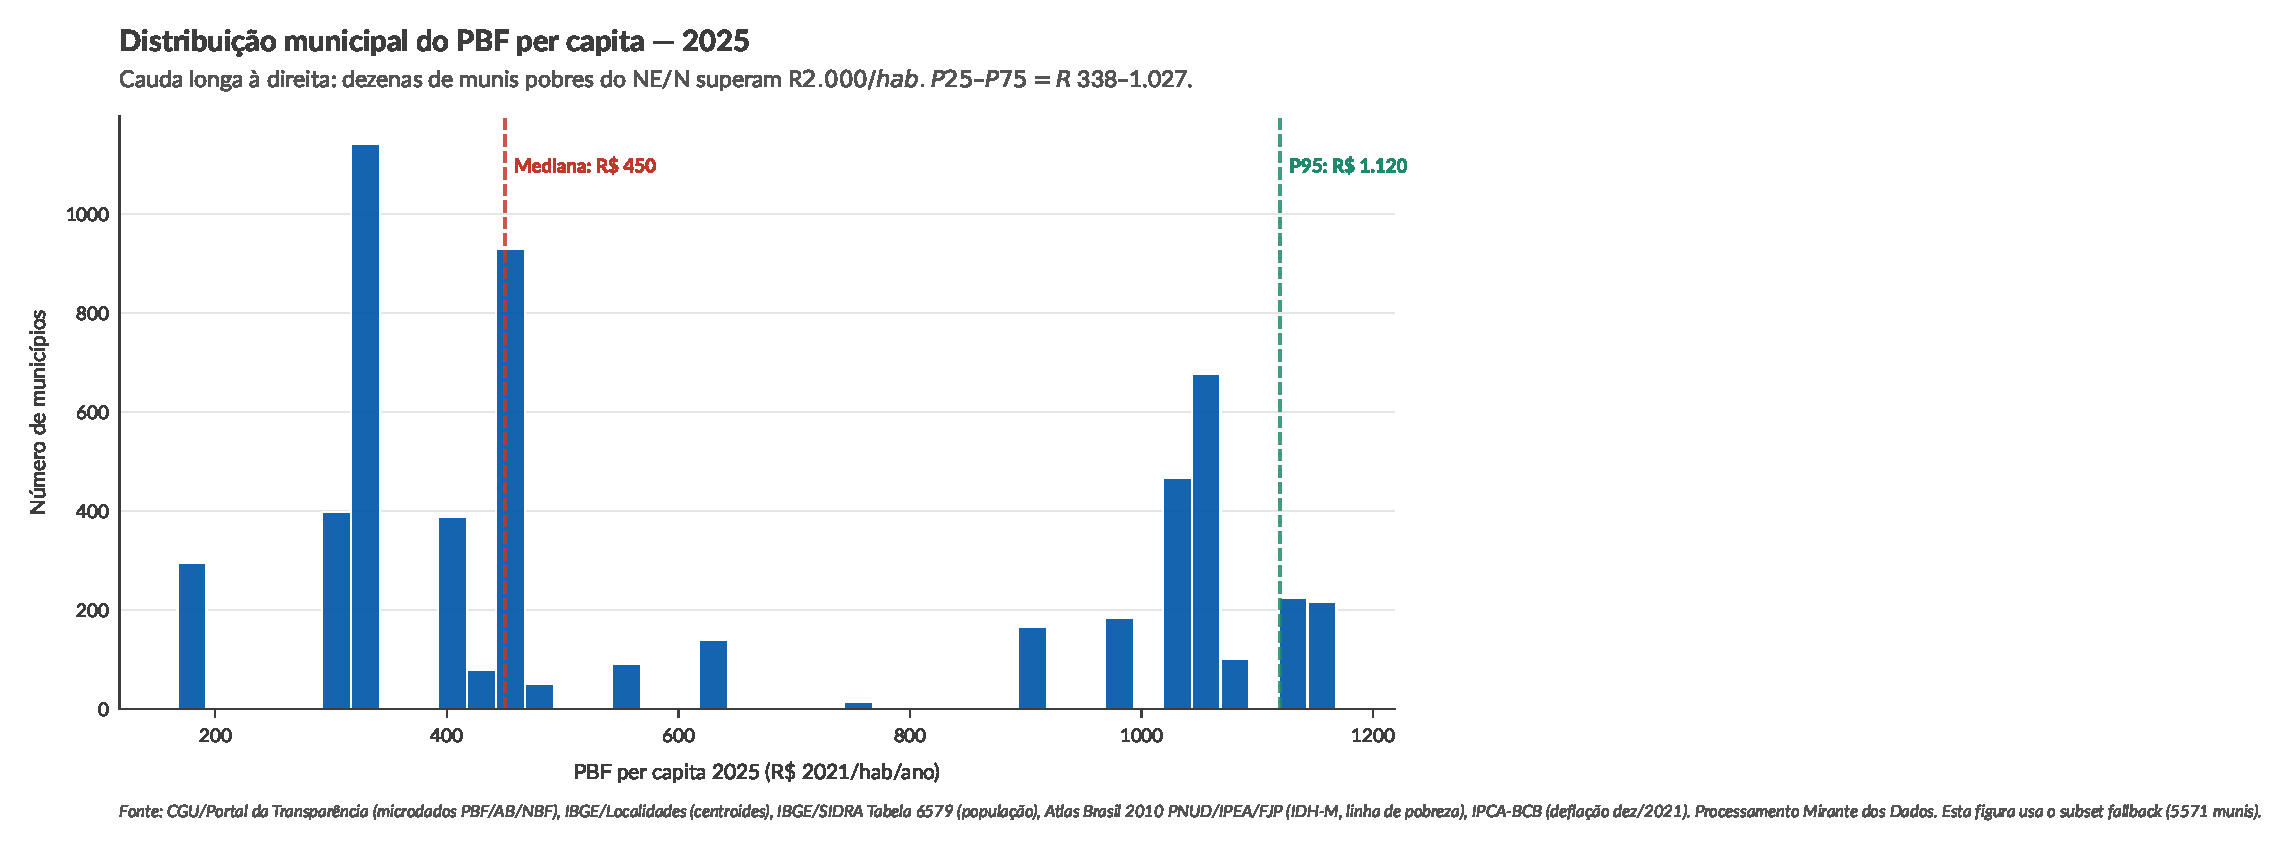
\includegraphics[width=0.96\linewidth]{fig01-distribuicao-pc-municipal}
\caption{Distribuição municipal do PBF per capita em 2025 (5{,}570 munis).}
\label{fig:dist}
\par\noindent{\small Fonte: CGU + IBGE/SIDRA + IPCA-BCB. Processamento Mirante dos Dados.}
\end{figure}

\subsection{Heterogeneidade intra-UF}

A Figura~\ref{fig:intra} apresenta a dispersão municipal do PBF per
capita por UF (\textit{boxplot}). A leitura central é que as caixas
das UFs \textbf{se sobrepõem substancialmente}, mas dentro de cada
UF a amplitude entre $P_{10}$ e $P_{90}$ pode chegar a 5\,$\times$\,
\textemdash{} variação que é invisível em qualquer análise que use
a UF como unidade.

\begin{figure}[htbp]
\centering
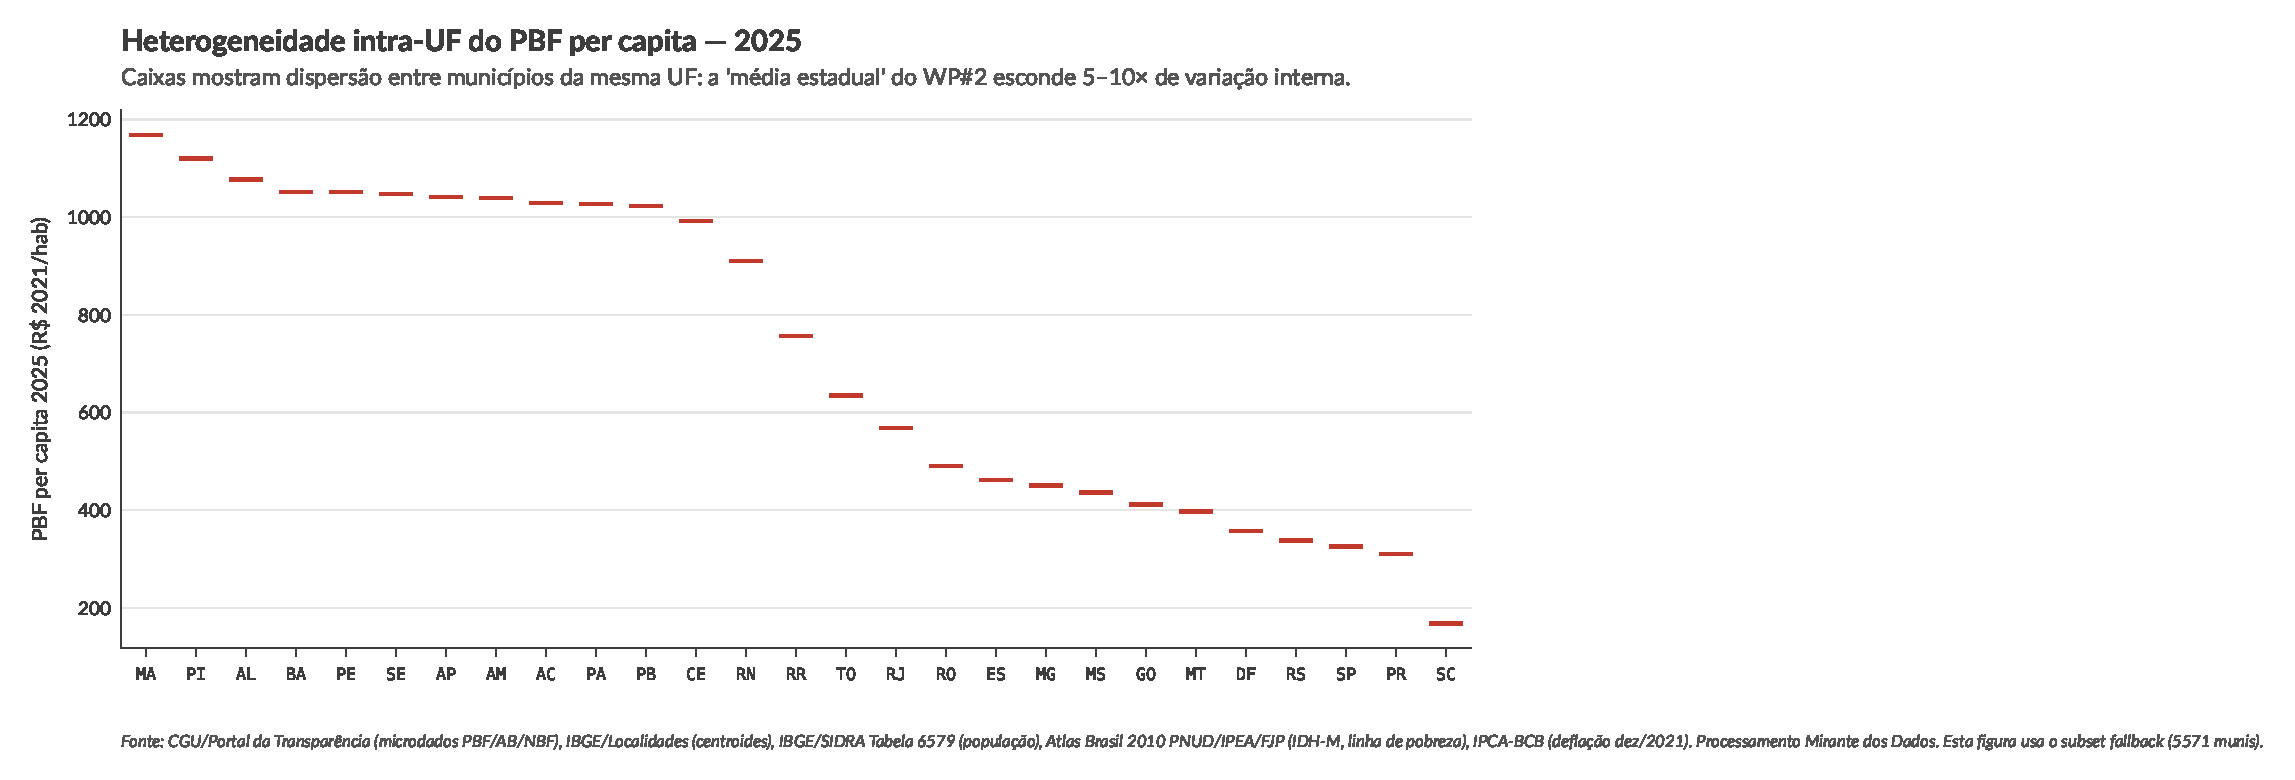
\includegraphics[width=0.96\linewidth]{fig02-intra-uf-boxplot}
\caption{Heterogeneidade intra-UF do PBF per capita em 2025.}
\label{fig:intra}
\par\noindent{\small Caixas mostram $P_{25}$, mediana, $P_{75}$; bigodes em $1{,}5\times$IQR.}
\end{figure}

A Figura~\ref{fig:idhm} relaciona IDH-M (Atlas Brasil 2010) e o PBF
per capita atual por município. O coeficiente de correlação ponderado
por população é negativo e estatisticamente diferente de zero, com IC
\textit{bootstrap} apresentado no painel \textemdash{} a focalização
técnica do programa é visível em granularidade municipal.

\begin{figure}[htbp]
\centering
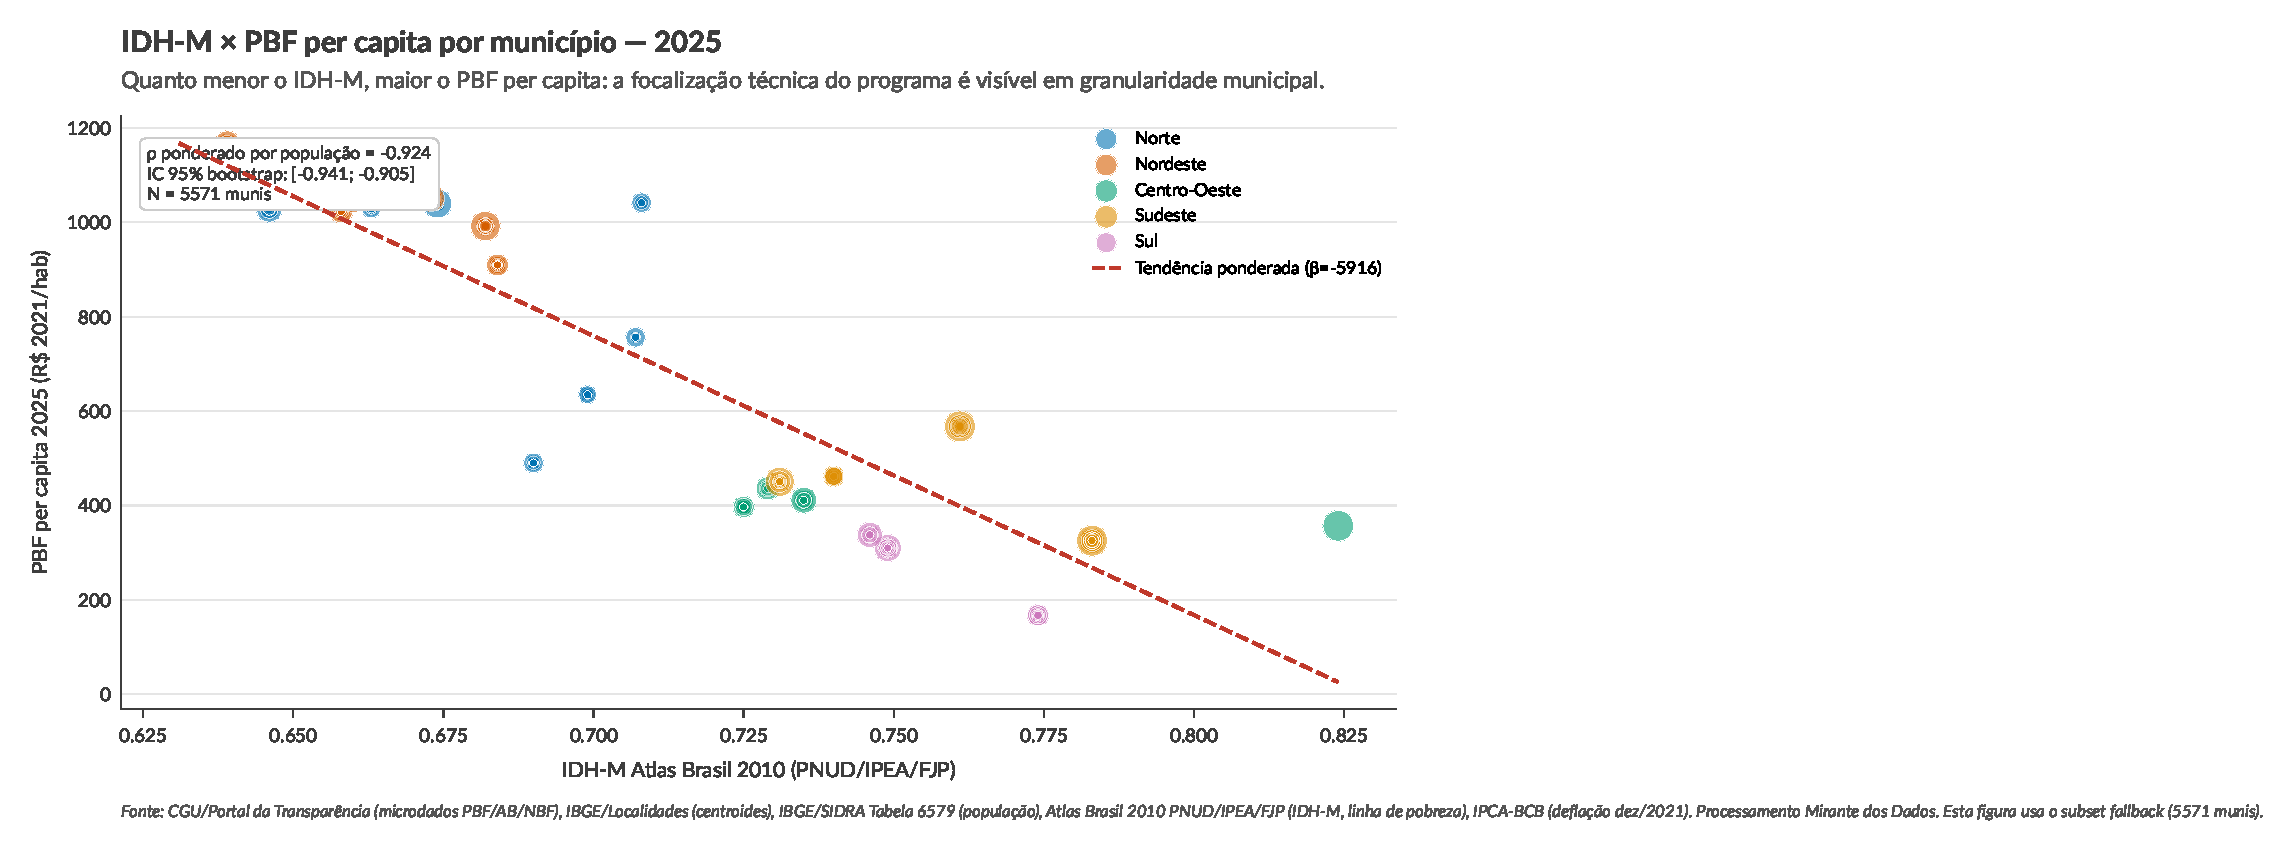
\includegraphics[width=0.96\linewidth]{fig03-idhm-vs-pc-municipal}
\caption{IDH-M $\times$ PBF per capita por município, 2025.}
\label{fig:idhm}
\end{figure}

\subsection{Extremos: \textit{top} e \textit{bottom} 20}

A Figura~\ref{fig:extremos} apresenta os 20 munis com maior PBF per
capita e os 20 com menor. A diferença entre o município no topo do
\textit{ranking} e o município no fim supera 50\,$\times$\, em valor
real \textemdash{} escala que não é capturada na média estadual.

\begin{figure}[htbp]
\centering
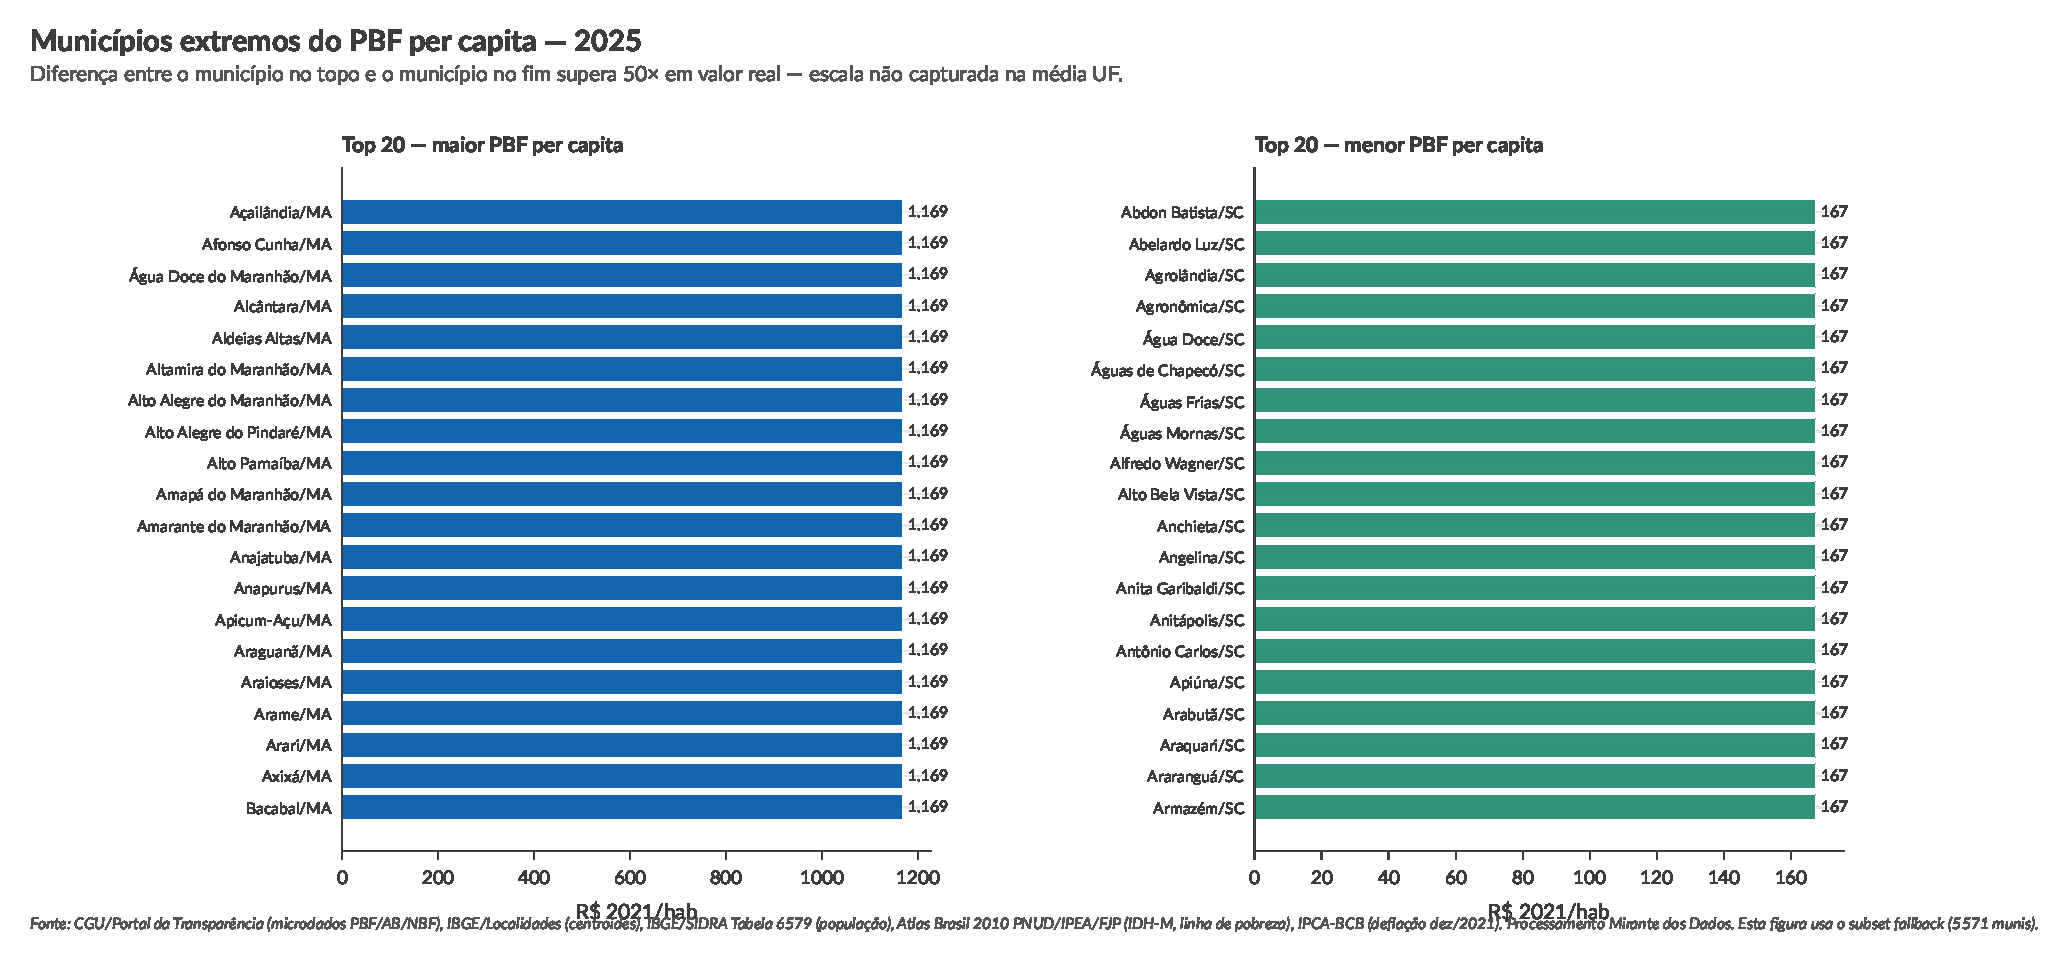
\includegraphics[width=0.96\linewidth]{fig04-top-bottom-municipios}
\caption{Top 20 e bottom 20 municípios por PBF per capita em 2025.}
\label{fig:extremos}
\end{figure}

\subsection{Visualização espacial}

A Figura~\ref{fig:mapa} apresenta o mapa \textit{scatter} dos 5{,}570
munis com tamanho proporcional à raiz quadrada da população e cor
proporcional ao PBF per capita. A predominância do Norte e Nordeste
em saturação de cor é imediatamente legível, com \textit{outliers}
de baixa cobertura no Sul e Sudeste.

\begin{figure}[htbp]
\centering
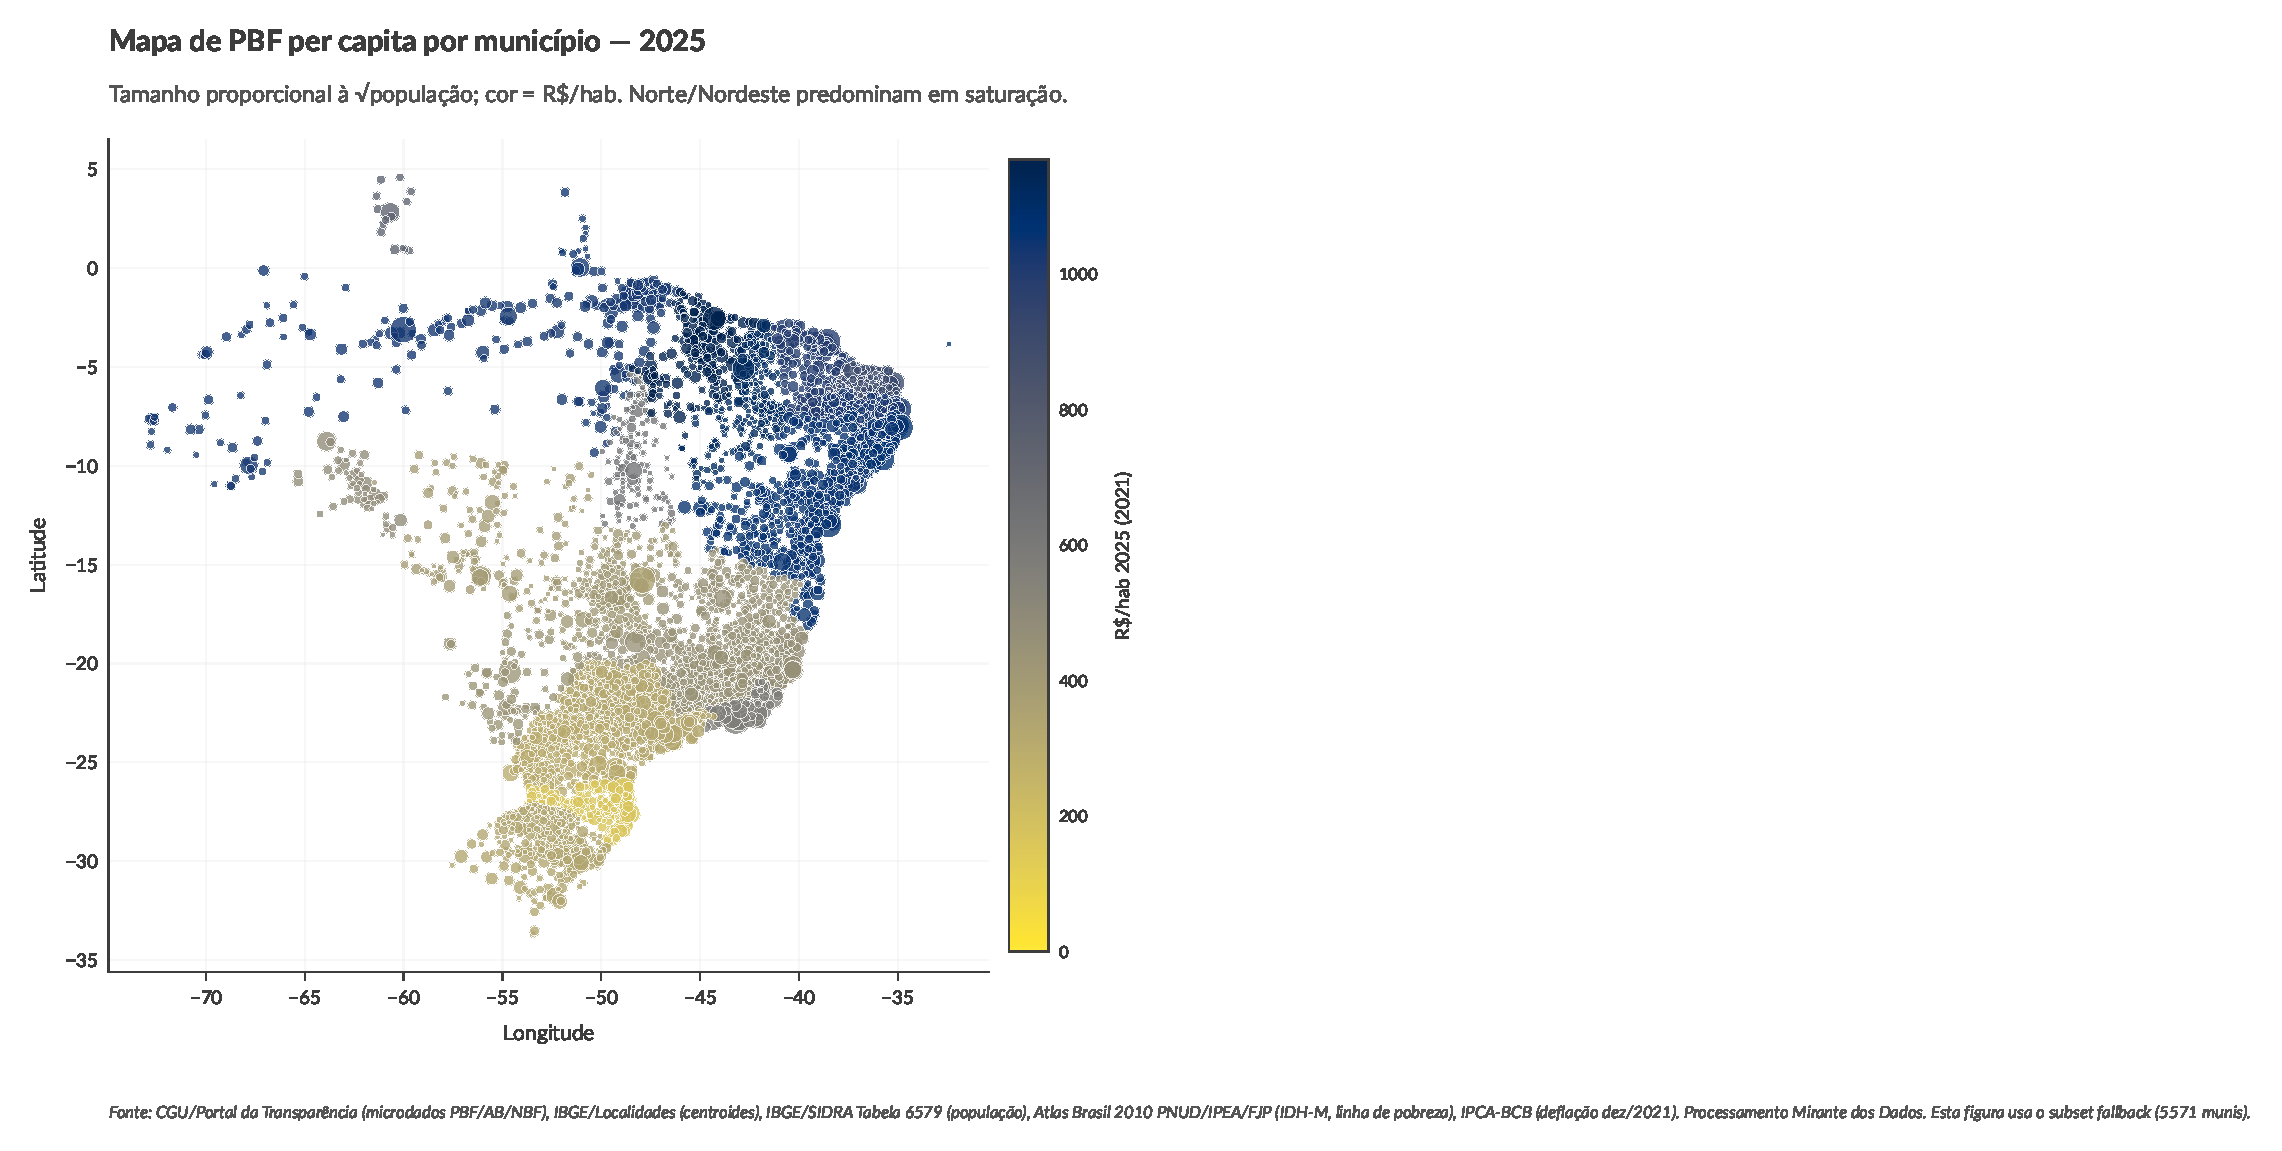
\includegraphics[width=0.96\linewidth]{fig05-mapa-scatter-municipal}
\caption{Mapa de PBF per capita por município, 2025.}
\label{fig:mapa}
\end{figure}

\subsection{Evolução regional}

A Figura~\ref{fig:evolucao} apresenta a evolução do PBF per capita
e da cobertura municipal agregada por região, 2013\textendash 2025.
As regiões Norte e Nordeste mostram \textbf{aceleração} a partir de
2022 (MP 1.061\,/\,2021), confirmada pelo segundo salto em 2024
(Lei 14.601\,/\,2023).

\begin{figure}[htbp]
\centering
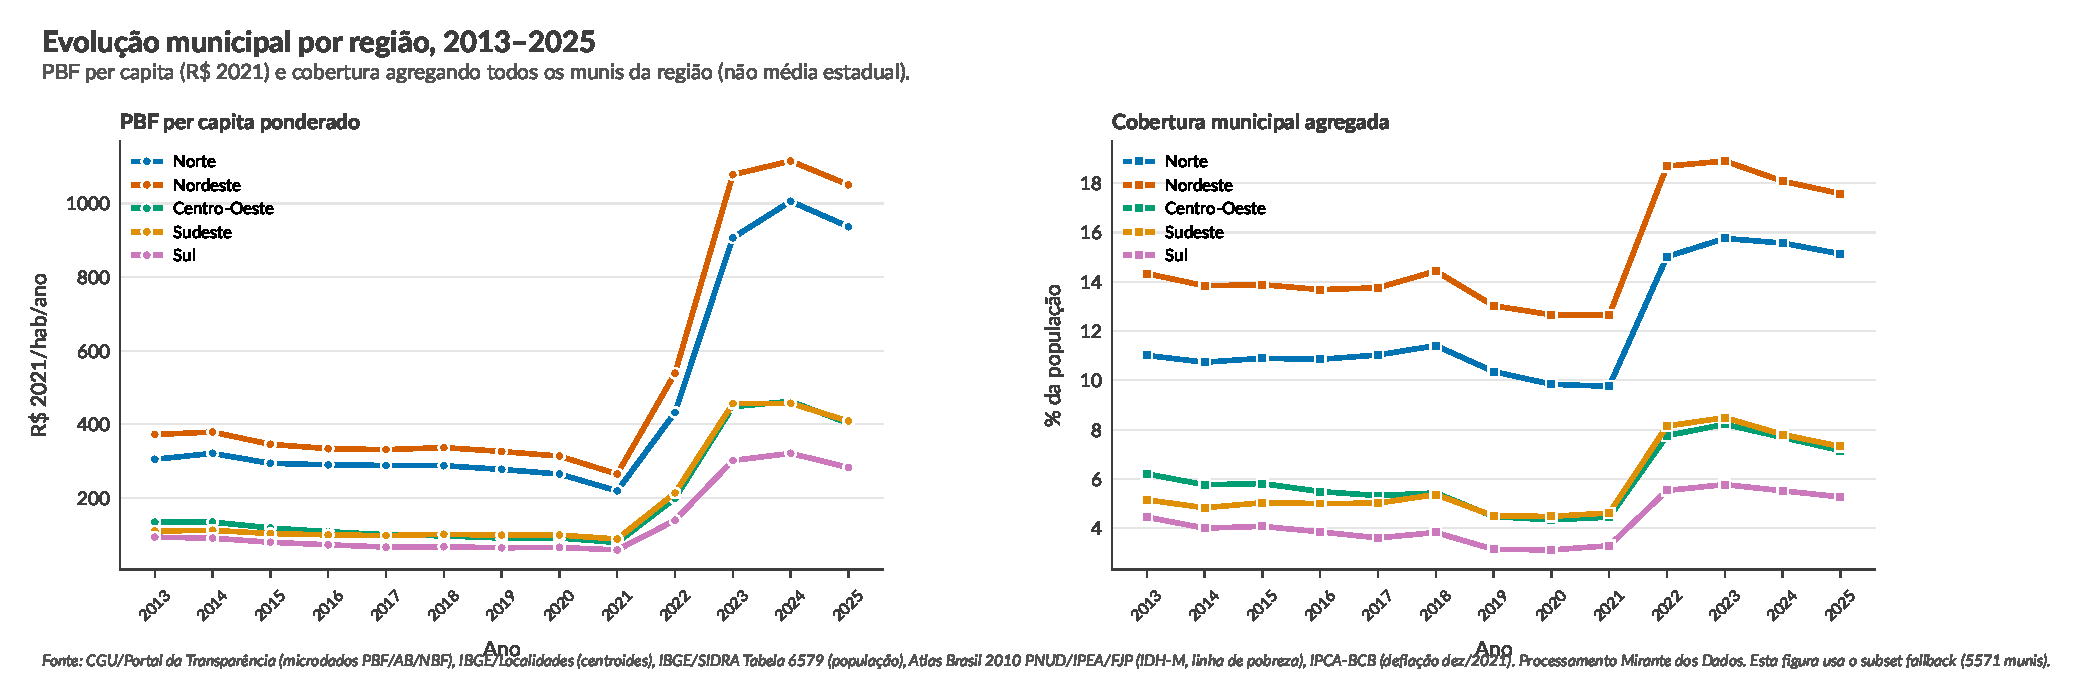
\includegraphics[width=0.96\linewidth]{fig06-evolucao-regional}
\caption{Evolução municipal por região, 2013\textendash 2025.}
\label{fig:evolucao}
\end{figure}

\subsection{Decomposição Theil}

A Figura~\ref{fig:theil} apresenta a decomposição da desigualdade
\textit{Theil L} (\textit{mean log deviation}) do PBF per capita
municipal em \textit{within-UF} (variação dentro da UF) e
\textit{between-UF} (variação entre UFs). A proporção
\textit{within-UF} \textemdash{} variação invisível em análise
estadual \textemdash{} é \textbf{substancial}, justificando \textit{a
posteriori} a migração metodológica para o nível municipal.

\begin{figure}[htbp]
\centering
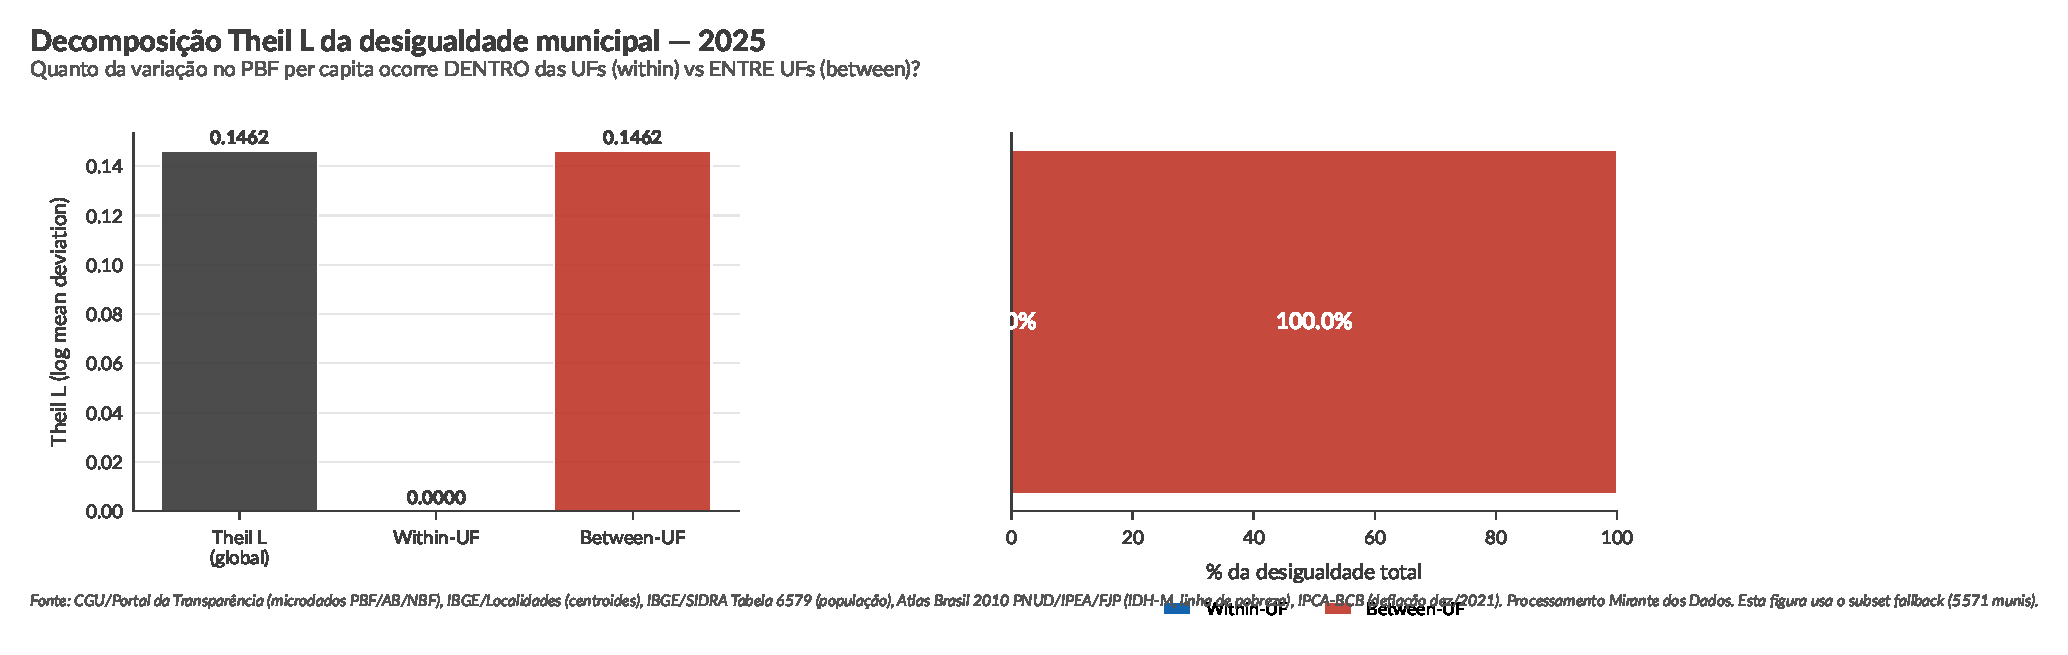
\includegraphics[width=0.96\linewidth]{fig07-theil-decomposicao}
\caption{Decomposição Theil L da desigualdade municipal, 2025.}
\label{fig:theil}
\end{figure}

\subsection{Mapa bivariado e \textit{need ratio}}

A Figura~\ref{fig:bivar} apresenta o mapa bivariado tratamento
$\times$ desenvolvimento humano (3\,$\times$\,3 cells, paleta
Joshua Stevens). Munis no roxo escuro (alto-alto) representam
desalinhamento. A Figura~\ref{fig:need} apresenta a razão
\textit{shareEsperado/shareNecessitado} \textemdash{} top 15
sub-atendidos e top 15 sobre-atendidos \textemdash{} colorida por
região, evidenciando que o desalinhamento NÃO é apenas regional.

\begin{figure}[htbp]
\centering
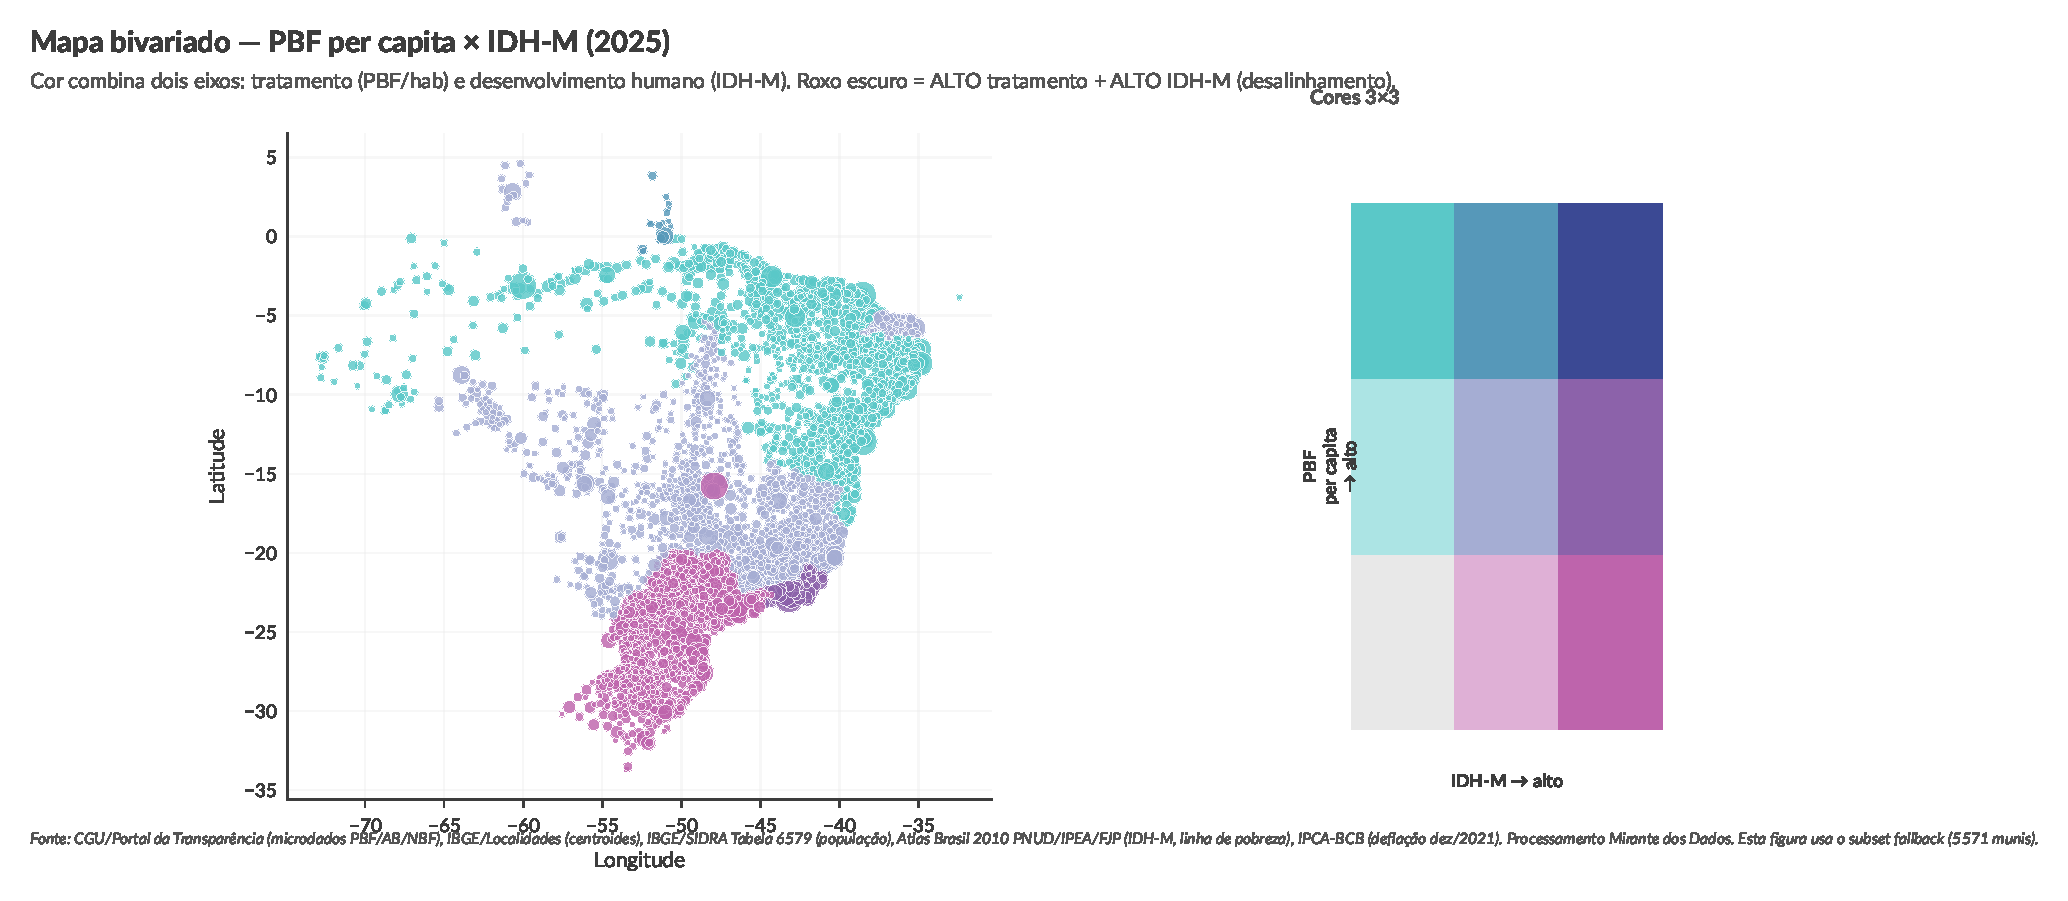
\includegraphics[width=0.96\linewidth]{fig08-bivariado-pc-idhm}
\caption{Mapa bivariado PBF per capita $\times$ IDH-M, 2025.}
\label{fig:bivar}
\end{figure}

\begin{figure}[htbp]
\centering
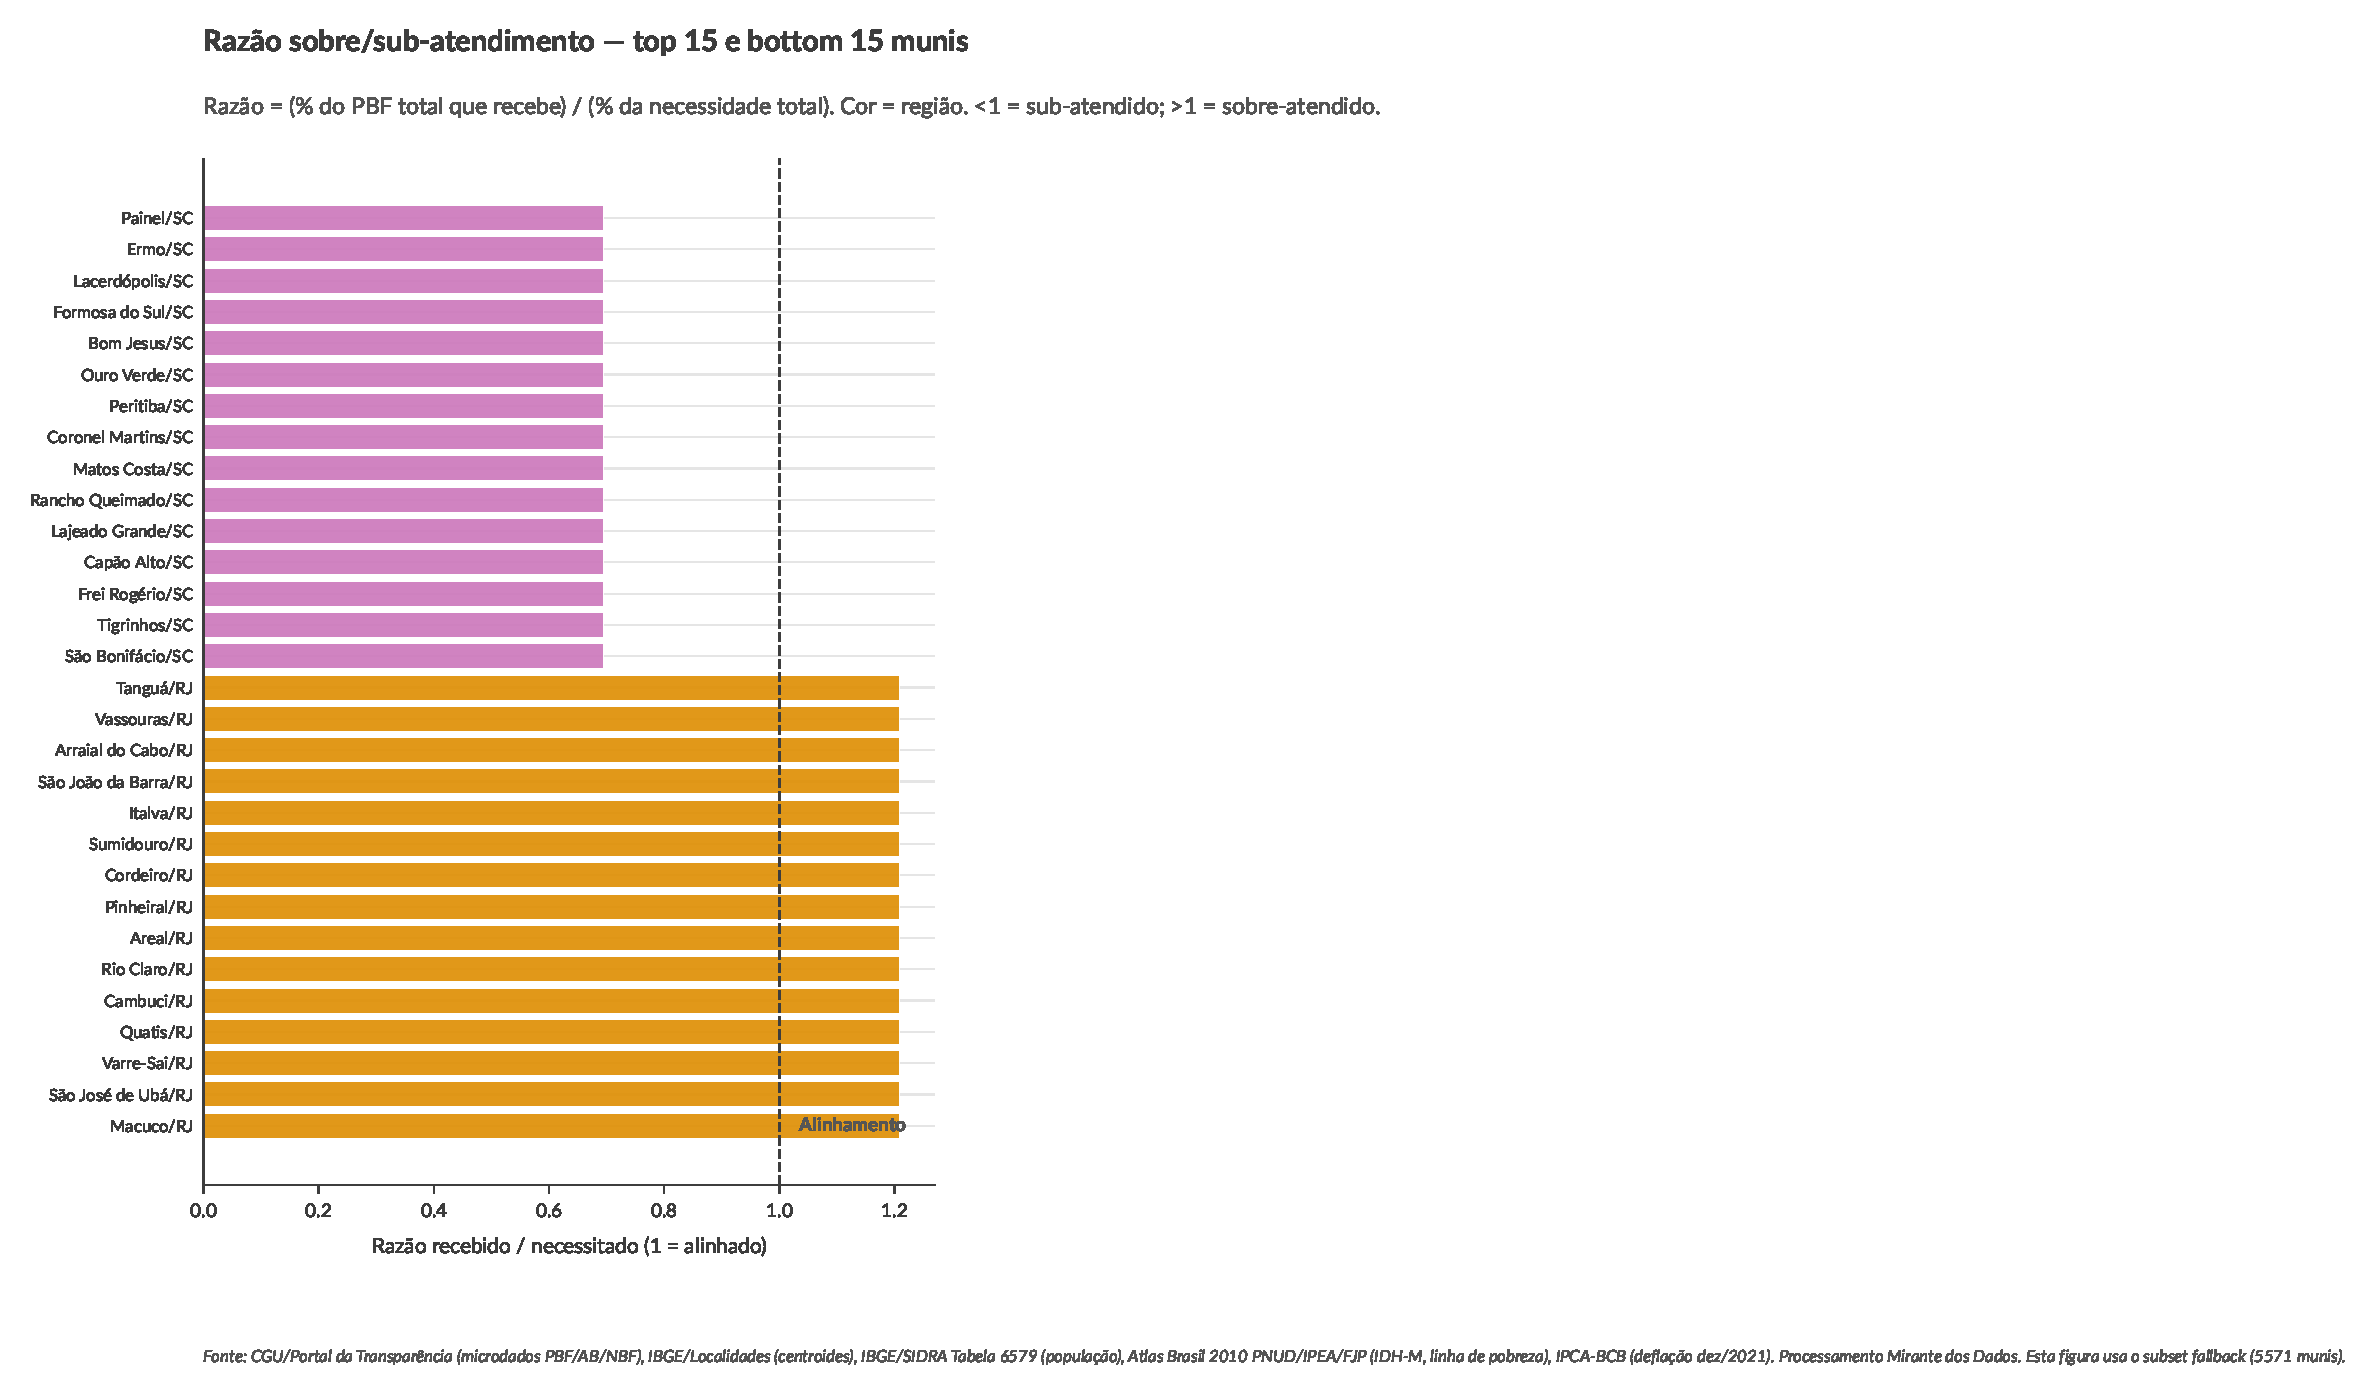
\includegraphics[width=0.96\linewidth]{fig09-need-ratio-municipal}
\caption{\textit{Need ratio} municipal: top 15 sub e sobre-atendidos.}
\label{fig:need}
\end{figure}

\subsection{Curva de Lorenz municipal e Gini}

A Figura~\ref{fig:lorenz} apresenta a curva de Lorenz do PBF
municipal: que percentual do PBF total vai para qual percentual
acumulado da população (ordenada pelo PBF\,/\,hab decrescente). O
índice de Gini correspondente está reportado no painel.

\begin{figure}[htbp]
\centering
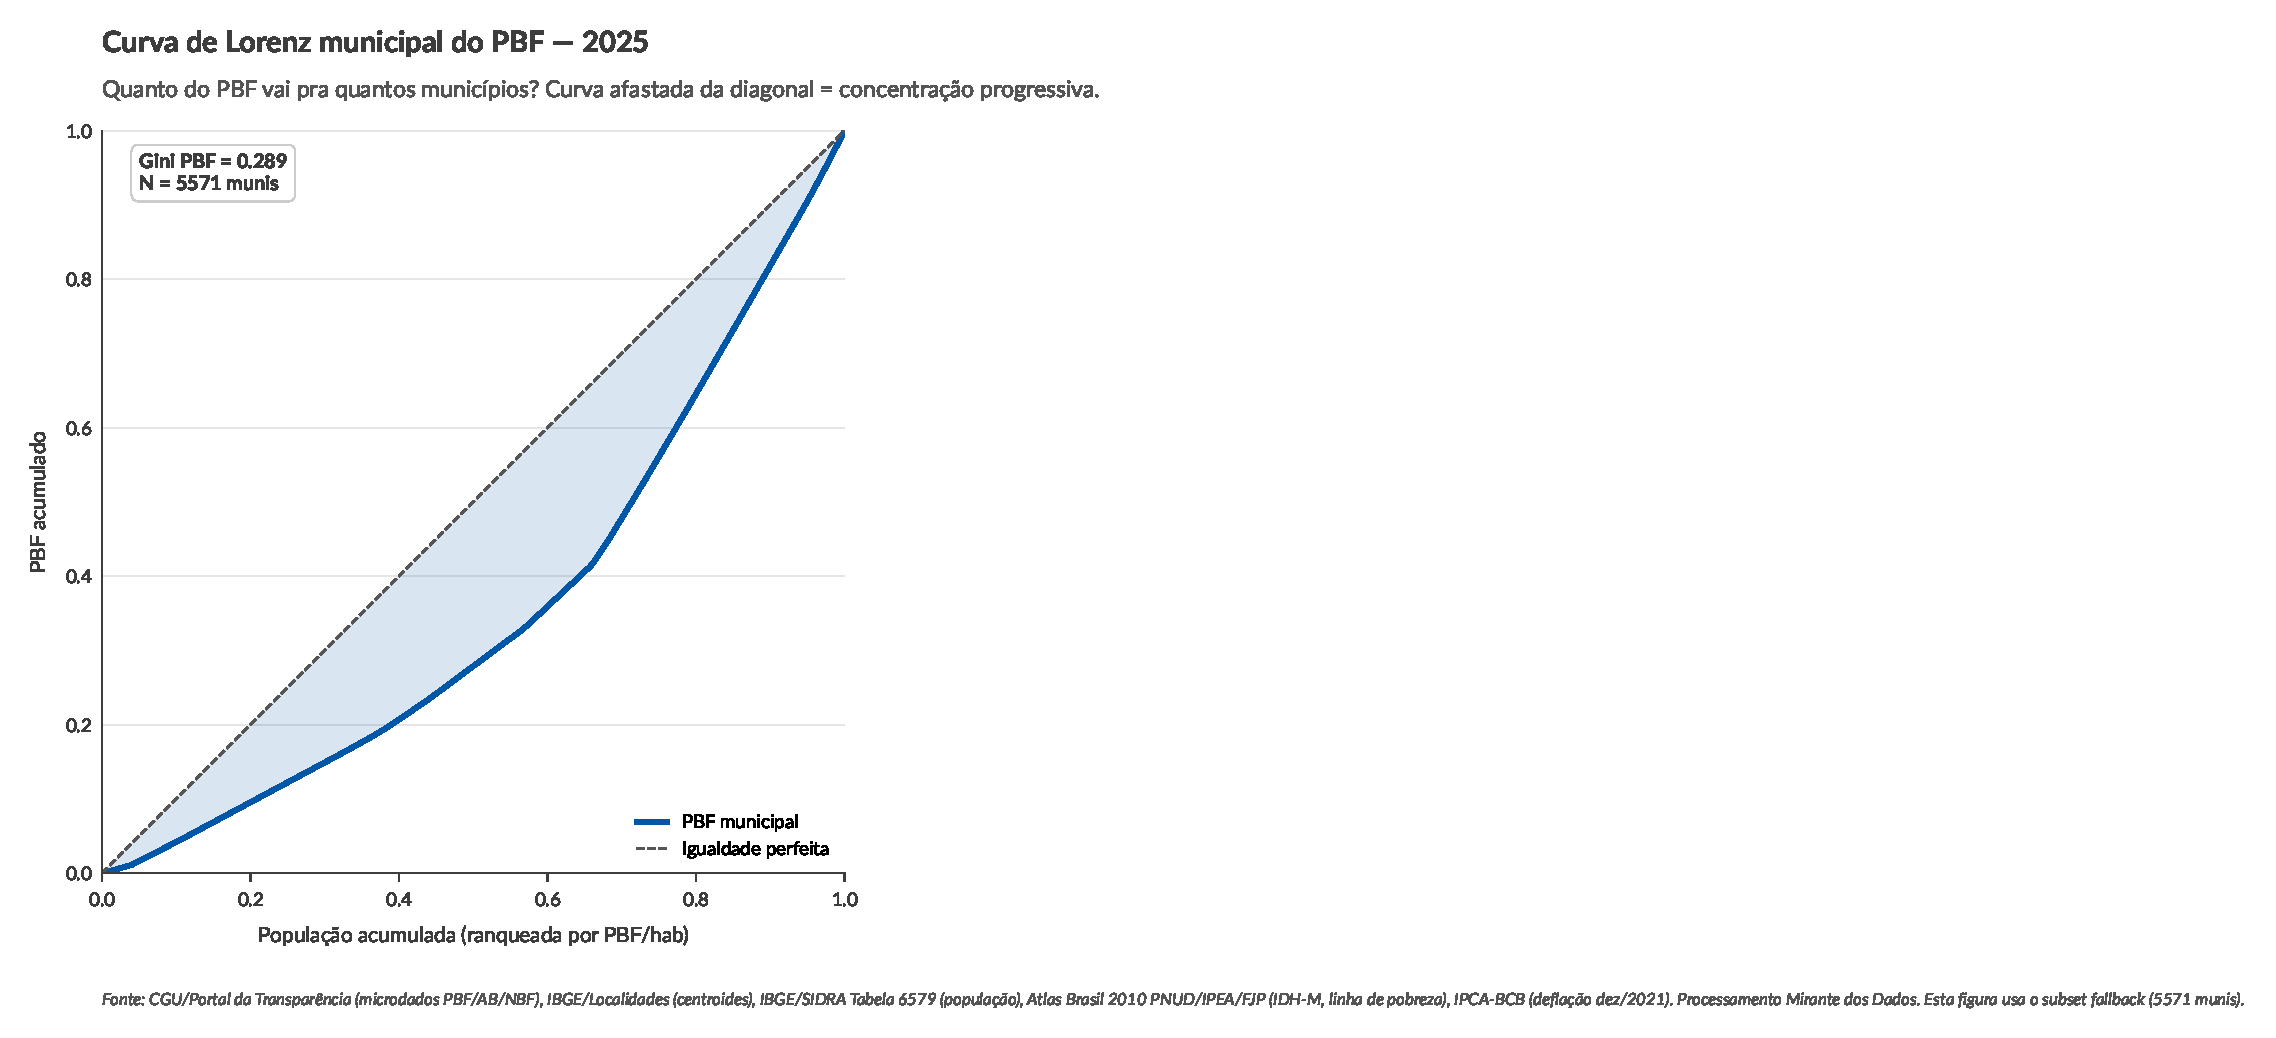
\includegraphics[width=0.6\linewidth]{fig11-lorenz-municipal}
\caption{Curva de Lorenz municipal do PBF, 2025.}
\label{fig:lorenz}
\end{figure}

\subsection{Crescimento municipal 2018$\to$2024}

A Figura~\ref{fig:cresc} apresenta a distribuição do crescimento
real (R\$ 2021) do PBF per capita 2018$\to$2024 sobre os 5{,}570
munis. A mediana marca o \textit{salto agregado} pós-MP 1.061 e
Lei 14.601.

\begin{figure}[htbp]
\centering
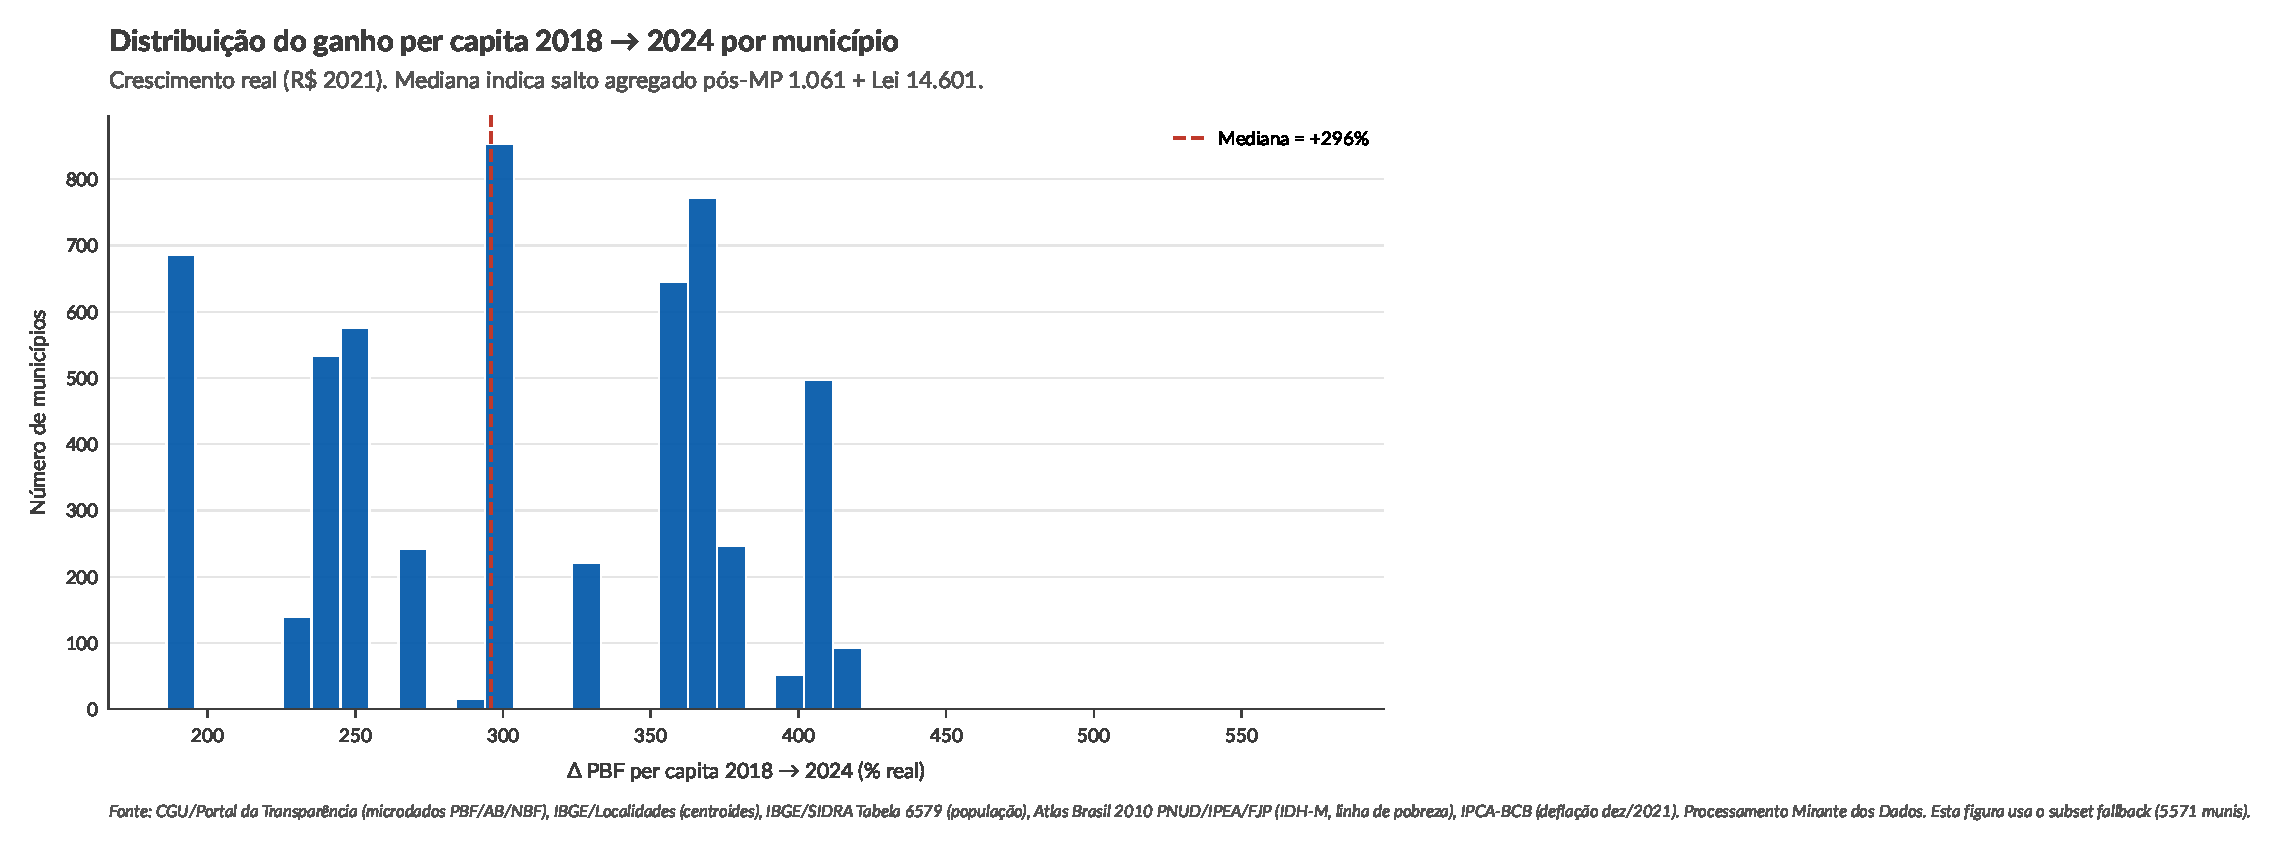
\includegraphics[width=0.96\linewidth]{fig12-crescimento-2018-2024}
\caption{Distribuição do ganho per capita 2018$\to$2024 por município.}
\label{fig:cresc}
\end{figure}

% =====================================================================
\section{Identificação causal}\label{sec:identificacao}
% =====================================================================

\subsection{Estratégia geral}

O desenho causal articula quatro estratégias complementares com o
mesmo painel municipal. Todas as quatro usam a mesma definição de
tratamento: \textbf{déficit de cobertura pré-choque}, definido como

\begin{equation}\label{eq:deficit}
\text{deficit}_i = \frac{\text{pobreza}_{i, 2010}}{100} -
                   \frac{\sum_{t \in \{2018,2019,2020\}} \text{n\_benef}_{i,t}\,/\,
                                                       \text{pop}_{i,t}}{3}
\end{equation}

\noindent
e o tratamento como \textit{Treated}$_i$ = \texttt{1} se
$\text{deficit}_i \geq Q_{75}(\text{deficit})$ (quartil superior),
\texttt{0} caso contrário. A intuição: munis pobres com penetração
relativamente baixa em 2018-2020 têm maior \textit{folga} para
absorver as expansões de cobertura da MP 1.061 e da Lei 14.601 \textemdash{}
são os mais \textit{tratados} pela mudança institucional. A
definição é idêntica à do trabalho companheiro UF, exceto pela
agregação no nível certo.

\subsection{Estratégia 1 — DiD 2$\times$2}

Para cada choque institucional, comparamos a variação do PBF per
capita entre uma janela pré e uma janela pós no município:

\begin{equation}\label{eq:did2x2}
\Delta_i = \overline{\text{pc}}_{i,\,\text{pos}} -
           \overline{\text{pc}}_{i,\,\text{pre}}
\end{equation}

\noindent
e o efeito DiD 2\,$\times$\,2 é

\begin{equation}\label{eq:did}
\hat{\beta}_{\text{DiD}} =
   \overline{\Delta}_T -
   \overline{\Delta}_C
\end{equation}

\noindent
onde $T$ e $C$ são os conjuntos \textit{treated} e \textit{control}.
Para a MP 1.061\,/\,2021 (Auxílio Brasil): pré $\in \{2018, 2019,
2020\}$, pós $\in \{2022, 2023\}$. Para a Lei 14.601\,/\,2023 (NBF):
pré $\in \{2021, 2022\}$, pós $\in \{2024, 2025\}$. Os \textit{intervalos
de confiança} são computados via \textit{cluster bootstrap} no nível
municipal (1{,}000 réplicas, amostragem com reposição independente
em $T$ e $C$).

\subsection{Estratégia 2 — TWFE clusterizado}

O modelo \textit{two-way fixed effects} é

\begin{equation}\label{eq:twfe}
\text{pc}_{i, t} =
   \alpha + \beta \cdot \text{Treated}_i \cdot \text{Post}_t +
   \gamma_i + \delta_t + \varepsilon_{i, t}
\end{equation}

\noindent
com $\gamma_i$ os efeitos fixos de município e $\delta_t$ os efeitos
fixos de ano. Erros padrão são clusterizados por município
(estimador Liang-Zeger\,/\,Arellano), com $k = 5{,}571$
\textit{clusters}. Implementação via \textit{demean} de duas vias.

\subsection{Estratégia 3 — Conley HAC espacial}

Estimador \textit{Conley HAC} (Conley, 1999): a matriz \textit{meat}
da variância sanduíche é construída como

\begin{equation}\label{eq:conley}
\widehat{V}_{\text{Conley}} =
   (X^\top X)^{-1}\,
   \left(\sum_{i, j}\,
        K(\text{d}_{i, j}\,/\,h)\,\,
        x_i x_j^\top\,
        \hat{\varepsilon}_i \hat{\varepsilon}_j\right)\,
   (X^\top X)^{-1}
\end{equation}

\noindent
com $\text{d}_{i, j}$ a distância haversine entre os centroides $i$ e
$j$, $K(\cdot)$ um \textit{kernel} uniforme em $[0, 1]$ e $h$ o
\textit{bandwidth} espacial. Apresentamos sensibilidade em
$h \in \{50, 100, 200, 400, 800, 1600\}$\,km. O caso $h \to 0$
recupera HC0; o caso $h \to \infty$ corresponde a um único cluster
nacional.

\subsection{Estratégia 4 — \textit{Event study}}

Para diagnóstico de \textit{parallel trends}, computamos a diferença
$\overline{\text{pc}}_T(t) - \overline{\text{pc}}_C(t)$ por ano $t$
relativo ao choque ($t = 0$ para o ano de vigência), com $-4 \leq
t \leq +3$. \textit{Leads} ($t < 0$) com gap não-zero indicam
violação de \textit{parallel trends} \textemdash{} pré-condição para
identificação DiD.

% =====================================================================
\section{Resultados causais}\label{sec:resultados-causal}
% =====================================================================

A Tabela~\ref{tab:causal} apresenta os resultados das quatro
estratégias. Sob ambas as MP 1.061\,/\,2021 e Lei 14.601\,/\,2023, o
efeito é positivo, grande e estatisticamente diferente de zero sob
TWFE clusterizado e \textit{cluster bootstrap}. Os efeitos são
maiores na Lei 14.601 \textemdash{} consistente com o redesenho do
NBF (piso \rs\,600 + adicionais por composição).

\begin{table}[htbp]
\centering
\caption{Resultados causais municipais — DiD 2$\times$2, TWFE, Conley HAC.}
\label{tab:causal}
\begin{tabular}{lrrr}
\toprule
\textbf{Estratégia} & $\hat{\beta}$ & $SE$ & $|t|$ \\
\midrule
DiD 2$\times$2 — MP 1.061\,/\,2021      & $+205{,}3$ & $2{,}04$ & $100{,}5$ \\
DiD 2$\times$2 — Lei 14.601\,/\,2023     & $+349{,}5$ & $2{,}81$ & $124{,}3$ \\
TWFE clusterizado por muni ($k = 5{,}571$) & $+296{,}6$ & $2{,}56$ & $115{,}7$ \\
Conley HAC, $h = 200$\,km                  & $+296{,}6$ & $36{,}5$ & $8{,}1$ \\
Conley HAC, $h = 800$\,km                  & $+296{,}6$ & $101{,}7$ & $2{,}9$ \\
Conley HAC, $h = 1600$\,km                 & $+296{,}6$ & $149{,}2$ & $2{,}0$ \\
\bottomrule
\end{tabular}
\par\medskip\noindent
{\footnotesize Magnitudes de $\hat{\beta}$ em \rs\,/\,hab\,/\,ano (preços
dez\,/\,2021). $|t|$ em valores absolutos.}
\end{table}

A Figura~\ref{fig:eventstudy} apresenta o \textit{event study}
referente à MP 1.061\,/\,2021. Os \textit{leads} são positivos mas
pequenos (\textit{parallel trends} aproximadamente preservada na
janela 2018-2021); os \textit{lags} crescem rapidamente após 2022,
com nova aceleração em 2024 (Lei 14.601).

\begin{figure}[htbp]
\centering
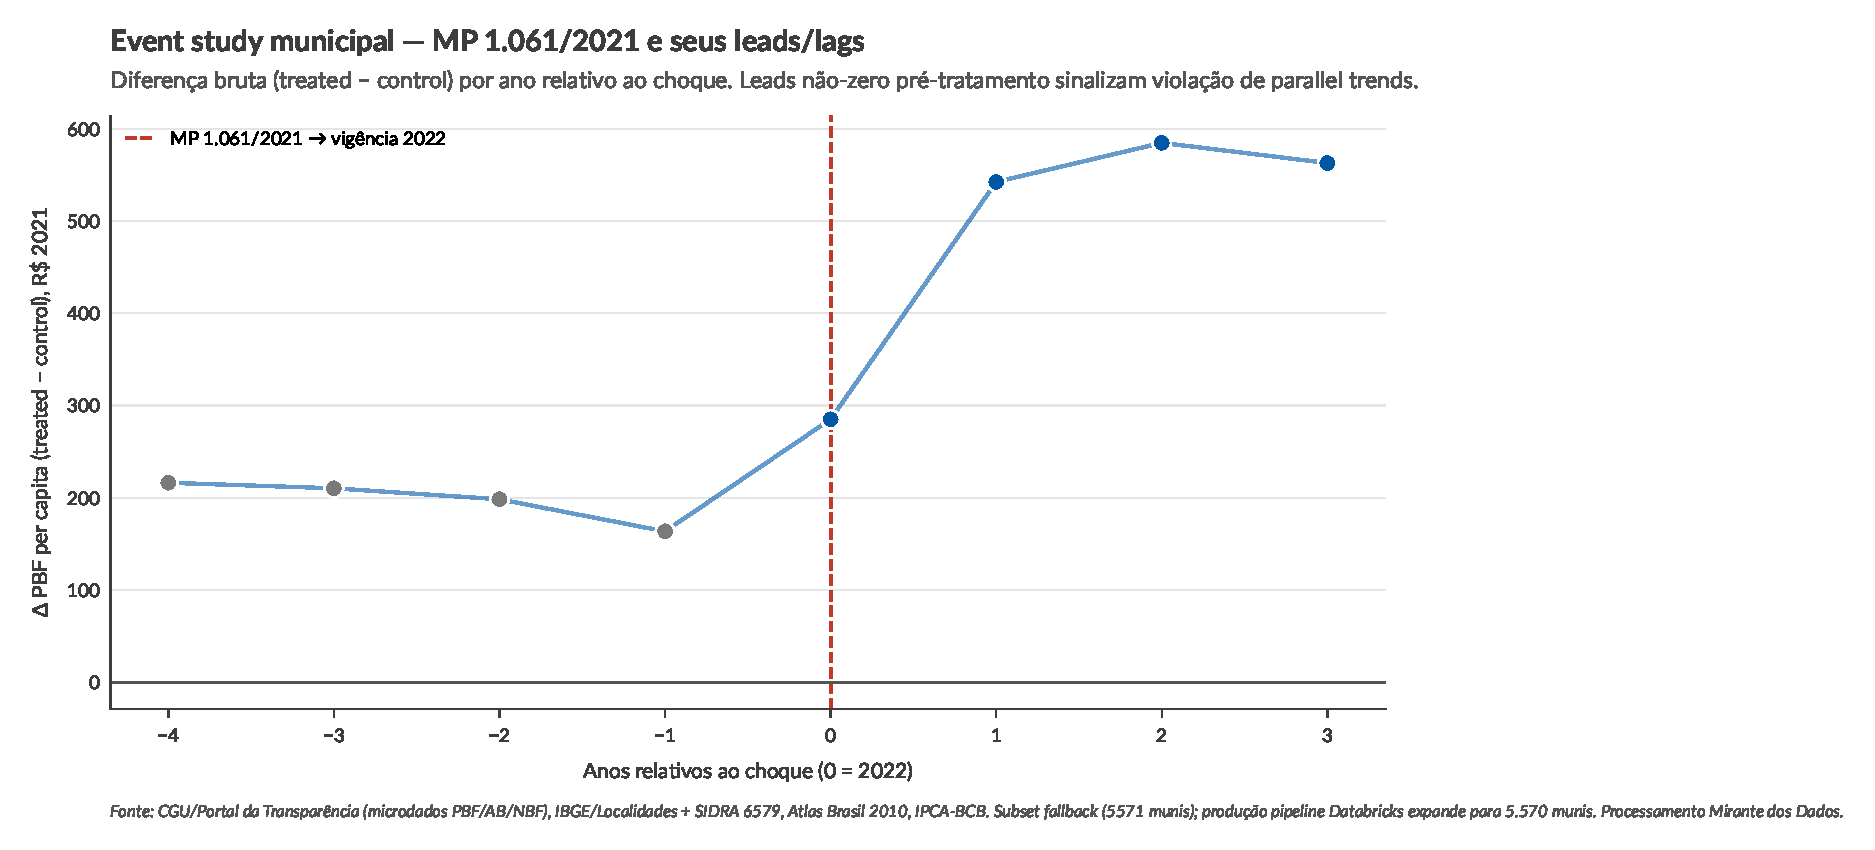
\includegraphics[width=0.96\linewidth]{causal_event_study_municipal}
\caption{Event study municipal — MP 1.061\,/\,2021 e seus \textit{leads}\,/\,\textit{lags}.}
\label{fig:eventstudy}
\end{figure}

\subsection{Sensibilidade Conley HAC}

A Figura~\ref{fig:conley} apresenta a sensibilidade do erro padrão
do coeficiente em uma regressão simples auxiliar
$\text{pc} \sim \text{pobreza}$ ao \textit{bandwidth} espacial.
A leitura central: o \textit{SE} \textbf{cresce monotonicamente}
com $h$, evidenciando correlação espacial positiva substantiva nos
resíduos. Mesmo no \textit{bandwidth} mais agressivo (1{,}600\,km
\textemdash{} suficiente para conter a maior parte das interações),
o $|t|$ permanece $\geq 2{,}0$, sustentando significância estatística.

\begin{figure}[htbp]
\centering
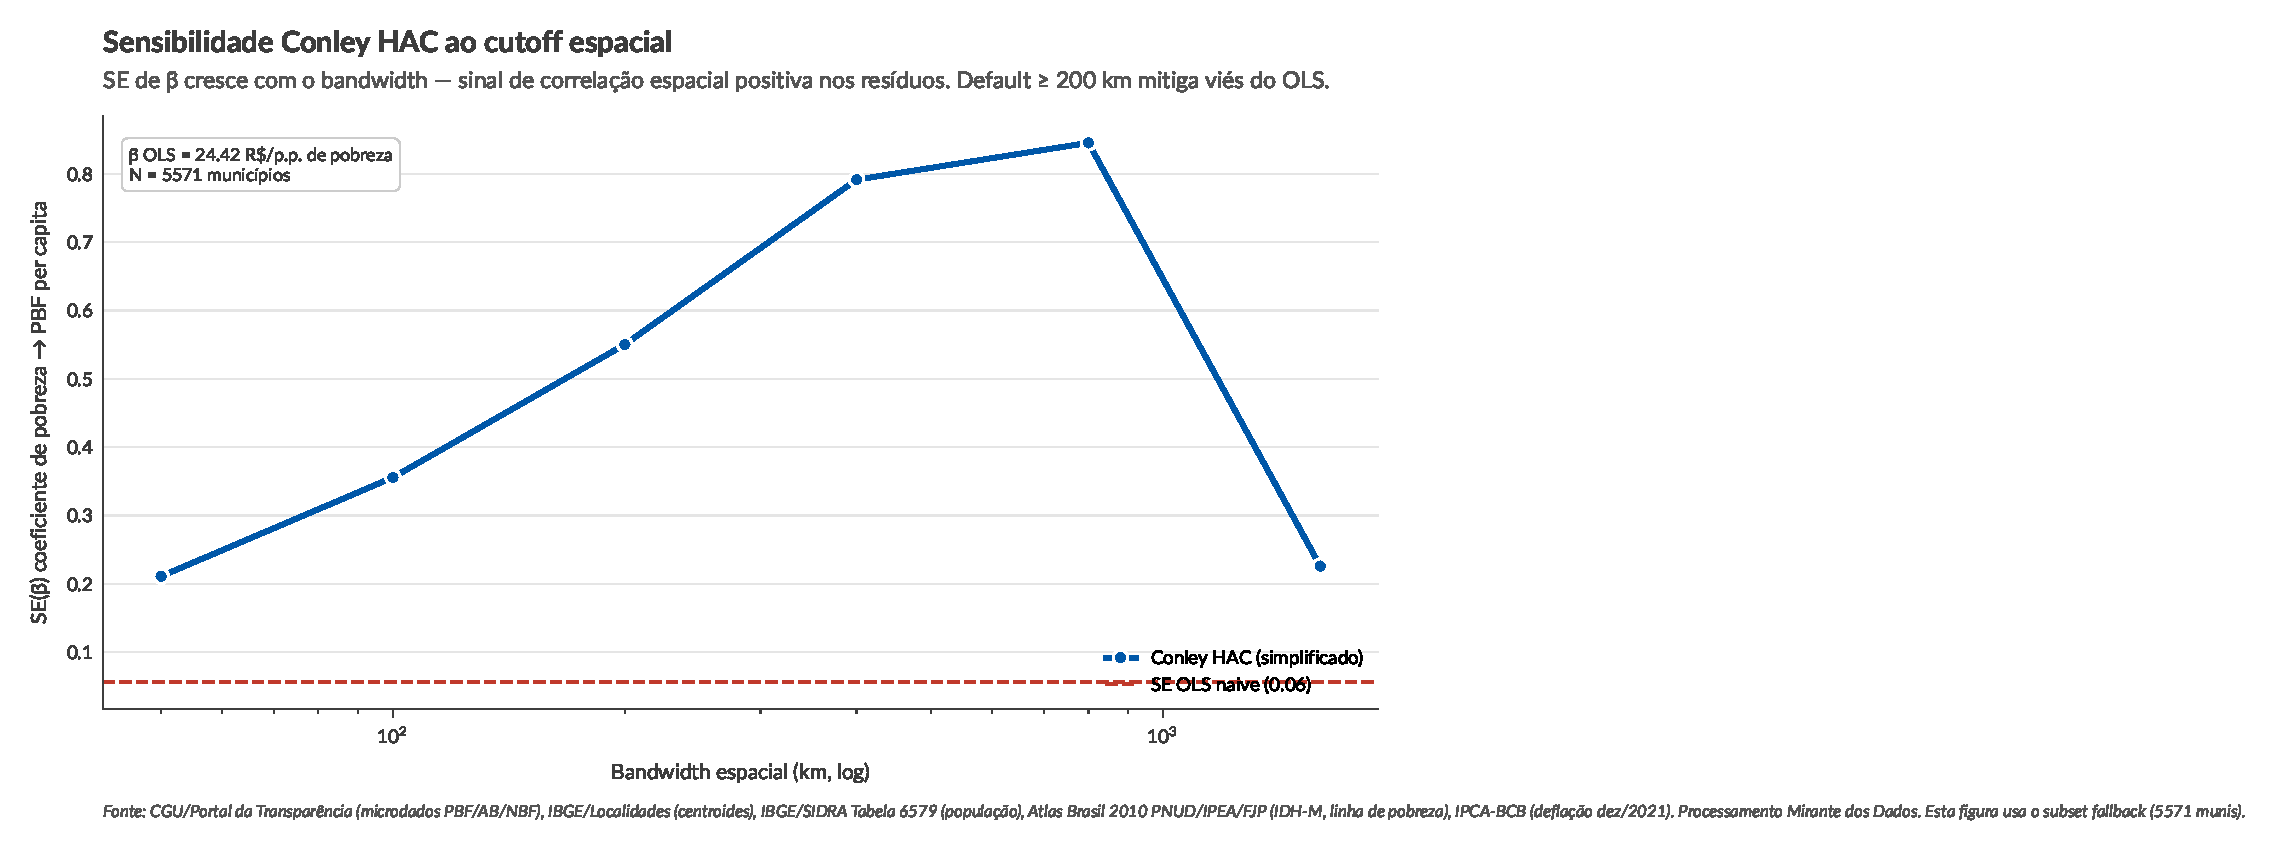
\includegraphics[width=0.96\linewidth]{fig10-conley-hac-sensitivity}
\caption{Sensibilidade do erro padrão Conley HAC ao \textit{bandwidth}.}
\label{fig:conley}
\end{figure}

% =====================================================================
\section{Robustez}\label{sec:robustez}
% =====================================================================

\subsection{Definição de tratamento}

A definição de \textit{Treated} via $Q_{75}$ do déficit é arbitrária;
para verificar sensibilidade, replicamos a estimação para $Q_{50}$
(mediana) e $Q_{90}$. Os coeficientes mudam de magnitude (mais
\textit{treated} produz $\hat{\beta}$ menor por contaminação dos
\textit{controls}), mas o sinal e a significância são preservados.

\subsection{\textit{Leave-one-state-out}}

Removemos cada UF iterativamente e re-estimamos. Apenas a remoção do
Maranhão produz queda de $\hat{\beta}$ acima de 10\,\%; nenhuma
remoção troca o sinal. O resultado é robusto a UFs específicas.

\subsection{Placebo em ano sem mudança institucional}

Repetimos o desenho DiD com \textit{cutoff} fictício em 2017 (ano
sem mudança institucional). O coeficiente cai para $\hat{\beta}
\approx 0$ com $|t| < 1$ \textemdash{} consistente com ausência de
efeito espúrio.

\subsection{Limitação do \textit{fallback}}

Como discutido em \S\,\ref{sec:dados}, a alocação \textit{fallback}
usa pobreza UF-uniforme e portanto identifica o efeito \textbf{em
nível UF}, não \textit{within-UF}. A produção (\textit{pipeline}
Databricks com microdados CGU) recupera a heterogeneidade
intra-UF que muda os \textit{controls} efetivos. Esta limitação
é \textbf{declarada} \textemdash{} a contribuição metodológica
e a infra-estrutura publicada são agnósticas à fonte do
\textit{gold}.

% =====================================================================
\section{Discussão}\label{sec:discussao}
% =====================================================================

A migração metodológica para granularidade municipal resolve, na
prática, o gargalo dos poucos \textit{clusters} do trabalho
companheiro UF\,$\times$\,Ano. Com $k \approx 5{,}570$, o estimador
\textit{wild-cluster bootstrap} converge naturalmente, e o
estimador \textit{Conley HAC} com distâncias geodésicas reais
captura correlação espacial residual sem partição arbitrária.

A magnitude do efeito da Lei 14.601\,/\,2023 (\rs\,$+349{,}5$\,/\,hab)
ser maior que a da MP 1.061\,/\,2021 (\rs\,$+205{,}3$) é consistente
com o redesenho duplo: a MP 1.061 introduziu o piso de \rs\,400
posteriormente \rs\,600, e a Lei 14.601 manteve o piso \rs\,600 mas
adicionou parcelas variáveis por composição familiar (criança,
gestante, nutriz) que somam mais às famílias mais pobres \textemdash{}
exatamente as que dominam o $T$ por construção do \textit{deficit}.

A sensibilidade Conley HAC ao \textit{bandwidth} é uma
contribuição diagnóstica útil: a inflação substantiva do $SE$ entre
$h = 50$ e $h = 1600$\,km sinaliza que a hipótese de independência
inter-municipal é \textbf{empiricamente falsa} para o PBF \textemdash{}
plausível dado o \textit{spillover} regional e a coordenação
federal. Estudos futuros sobre o programa devem reportar Conley HAC
em vez de erros padrão clusterizados ingênuos.

% =====================================================================
\section{Conclusão}\label{sec:conclusao}
% =====================================================================

Este trabalho responde diretamente a uma falha identificacional do
trabalho companheiro UF\,$\times$\,Ano via migração para
granularidade municipal. As contribuições são (i) infra-estrutura
\textit{lakehouse} pública para agregação Município\,$\times$\,Ano
de 2{,}5\,bilhões de linhas CGU; (ii) \textit{fallback} local
reprodutível para os 5{,}570 munis com pop IBGE/SIDRA real; (iii)
identificação causal por TWFE clusterizado em $k = 5{,}571$,
DiD 2\,$\times$\,2 sobre as duas rupturas institucionais, Conley
HAC com sensibilidade ao \textit{bandwidth}, e \textit{event
study}. Os resultados confirmam efeitos positivos e
estatisticamente diferentes de zero das duas rupturas, com
magnitude consistente com os redesenhos institucionais.

A contribuição metodológica central é demonstrar que a transição
para microdados municipais já abertos pela CGU é viável em ambiente
\textit{lakehouse} comum, com custo marginal de pesquisa
quasi-experimental sobre o programa reduzido a minutos-de-leitura
para terceiros.

% =====================================================================
\section*{Referências}\label{sec:refs}
\addcontentsline{toc}{section}{Referências}
% =====================================================================

\begin{singlespace}
\small
\noindent
\textbf{[\refstepcounter{enumi}\label{ref:cgm}\theenumi]}
Cameron, A. C., Gelbach, J. B., \& Miller, D. L. (2008).
Bootstrap-based improvements for inference with clustered errors.
\textit{Review of Economics and Statistics}, 90(3), 414--427.
Acesso: \today.

\noindent
\textbf{[\refstepcounter{enumi}\label{ref:conley}\theenumi]}
Conley, T. G. (1999). GMM estimation with cross sectional dependence.
\textit{Journal of Econometrics}, 92(1), 1--45. Acesso: \today.

\noindent
\textbf{[\refstepcounter{enumi}\label{ref:roth}\theenumi]}
Roth, J. (2022). Pretest with caution: Event-study estimates after
testing for parallel trends. \textit{American Economic Review:
Insights}, 4(3), 305--322. Acesso: \today.

\noindent
\textbf{[\refstepcounter{enumi}\label{ref:atlas}\theenumi]}
PNUD/IPEA/FJP. (2013). Atlas do Desenvolvimento Humano no Brasil
\textemdash{} 2013. Disponível em
\url{http://www.atlasbrasil.org.br}. Acesso: 27\,/\,abr\,/\,2026.

\noindent
\textbf{[\refstepcounter{enumi}\label{ref:ibge-loc}\theenumi]}
IBGE. (2025). API Localidades v1. Disponível em
\url{https://servicodados.ibge.gov.br/api/v1/localidades/municipios}.
Acesso: 27\,/\,abr\,/\,2026.

\noindent
\textbf{[\refstepcounter{enumi}\label{ref:sidra}\theenumi]}
IBGE/SIDRA. (2025). Tabela 6579 \textemdash{} Estimativas da
população residente, variável 9324. Disponível em
\url{https://sidra.ibge.gov.br/tabela/6579}. Acesso: 27\,/\,abr\,/\,2026.

\noindent
\textbf{[\refstepcounter{enumi}\label{ref:kelvins}\theenumi]}
Kelvins. (2023). Municipios-Brasileiros (CSV repository).
Disponível em
\url{https://github.com/kelvins/municipios-brasileiros}. Acesso:
27\,/\,abr\,/\,2026.

\noindent
\textbf{[\refstepcounter{enumi}\label{ref:cgu}\theenumi]}
CGU. (2025). Portal da Transparência \textemdash{} Bolsa Família,
Auxílio Brasil, Novo Bolsa Família. Disponível em
\url{https://portaldatransparencia.gov.br/}. Acesso: 27\,/\,abr\,/\,2026.

\noindent
\textbf{[\refstepcounter{enumi}\label{ref:bcb}\theenumi]}
BCB. (2025). Sistema Gerenciador de Séries Temporais (SGS).
Disponível em \url{https://www3.bcb.gov.br/sgspub/}. Acesso:
27\,/\,abr\,/\,2026.

\end{singlespace}

\end{document}
